\documentclass[12pt,a4paper]{report}

% ==============================================================================
% PACKAGES AND SETUP
% ==============================================================================
\usepackage[utf8]{inputenc}
\usepackage[margin=1in]{geometry}
\usepackage{setspace}
\onehalfspacing

\usepackage{graphicx}
\usepackage{amsmath,amssymb,amsfonts}
\usepackage{booktabs}
\usepackage{array}
\usepackage{tabularx}
\usepackage{float}
\usepackage{tikz}
\usetikzlibrary{shapes.geometric, arrows.meta, positioning, calc}
\usepackage{titlesec}
\usepackage{fancyhdr}
\usepackage[hidelinks]{hyperref}
\usepackage{caption}
\usepackage{subcaption}
\usepackage{listings}
\usepackage{xcolor}

\lstset{
  basicstyle=\ttfamily\small,
  breaklines=true,
  frame=single,
  backgroundcolor=\color{gray!10},
  showstringspaces=false
}

% Chapter heading formatting
\titleformat{\chapter}[display]
  {\normalfont\huge\bfseries\centering}{\chaptertitlename\ \thechapter}{16pt}{\Huge}
\titlespacing*{\chapter}{0pt}{0pt}{20pt}

% Header and Footer
\pagestyle{fancy}
\fancyhf{}
\fancyfoot[C]{\thepage}
\renewcommand{\headrulewidth}{0pt}

% ==============================================================================
% DOCUMENT BEGINS
% ==============================================================================
\begin{document}

% ------------------------------------------------------------------------------
% TITLE PAGE
% ------------------------------------------------------------------------------
\begin{titlepage}
\centering
\vspace*{0.5cm}

{\LARGE \textbf{AegisFL: A Byzantine-Robust Federated Intrusion Detection Framework with Class-Aware Reputation and Blockchain Auditing}}\\[1.8cm]

{\large \textbf{Project Report submitted in partial fulfilment of}}\\[0.3cm]
{\large \textbf{Bachelor of Technology (B.Tech) in}}\\[0.3cm]
{\large \textbf{Computer Engineering (CE)}}\\[1.2cm]

{\large \textbf{by}}\\[0.4cm]
{\large \textbf{Dhruv Shrivastava (70022300545)}}\\[0.2cm]
{\large \textbf{Kritesh Goud (70022300195)}}\\[0.2cm]
{\large \textbf{Pratham Mourya (70022300207)}}\\[1.5cm]

{\large \textbf{Under the supervision of}}\\[0.3cm]
{\large \textbf{Dr. Vikas Kumar Jain}}\\[0.15cm]
{\normalsize (Assistant Professor, STME, Indore Campus)}\\[1.6cm]

{\large \textbf{SVKM's NMIMS University}}\\[0.15cm]
{\normalsize (Deemed-to-be University)}\\[0.6cm]


\begin{tikzpicture}
  \draw[thick, fill=gray!20] (0,0) rectangle (2.2,2.2);
  \node at (1.1,1.1) {\textbf{\large NMIMS}};
\end{tikzpicture}\\[0.6cm]

{\normalsize \textbf{SCHOOL OF TECHNOLOGY MANAGEMENT \& ENGINEERING (STME)}}\\[0.2cm]
{\normalsize \textbf{2026--27}}

\end{titlepage}

% ------------------------------------------------------------------------------
% CERTIFICATE
% ------------------------------------------------------------------------------
\newpage
\pagenumbering{roman}
\setcounter{page}{2}

\begin{center}
    {\Large \textbf{CERTIFICATE}}\\[1.2cm]
    
\begin{tikzpicture}
      \draw[thick, fill=gray!20] (0,0) rectangle (1.8,1.8);
      \node at (0.9,0.9) {\textbf{NMIMS}};
    \end{tikzpicture}\\[0.4cm]
    {\large \textbf{SVKM's NMIMS University}}\\[0.1cm]
    {\normalsize (Deemed-to-be University)}\\[1.2cm]
\end{center}

\noindent This is to certify that the project entitled \textbf{(AegisFL: A Byzantine-Robust Federated Intrusion Detection Framework with Class-Aware Reputation and Blockchain Auditing)}, has been done by \textbf{Dhruv Shrivastava} (SAP: 70022300545), \textbf{Kritesh Goud} (SAP: 70022300195), and \textbf{Pratham Mourya} (SAP: 70022300207) under my guidance and supervision \& has been submitted in partial fulfilment of the degree of \textbf{B.Tech in (Computer Engineering)} of STME, SVKM's NMIMS (Deemed-to-be University), Indore Campus, India.\\[2.5cm]

\noindent
\begin{minipage}{0.48\textwidth}
\textbf{Dr. Vikas Kumar Jain}\\
(Internal Guide)
\end{minipage}
\hfill
\begin{minipage}{0.48\textwidth}
\raggedleft
\textbf{Examiner}\\
(External)
\end{minipage}\\[3.0cm]

\noindent
\begin{minipage}{0.48\textwidth}
\textbf{Dr. Vikas Khare}\\
(Associate Dean, STME)
\end{minipage}\\[1.8cm]

\noindent \textbf{Date:} \rule{4cm}{0.4pt} \hfill \textbf{Place:} Indore

% ------------------------------------------------------------------------------
% ABSTRACT
% ------------------------------------------------------------------------------
\newpage
\chapter*{Abstract}
\addcontentsline{toc}{chapter}{Abstract}

Federated Learning (FL) enables geographically distributed network edge devices and organizations to collaboratively train an Intrusion Detection System (IDS) without centralizing raw traffic captures, ensuring compliance with global privacy regulations such as GDPR and India's Digital Personal Data Protection (DPDP) Act. However, standard aggregation protocols such as Federated Averaging (FedAvg) operate under an implicit honest-majority assumption. In real-world enterprise deployments, this assumption fails catastrophically under Byzantine model poisoning, adaptive gradient mimicry, and coordinated multi-client collusion, where malicious clients subtly degrade classification boundaries without triggering coarse global filters.

This project presents \textbf{AegisFL}, a comprehensive, Byzantine-robust federated intrusion detection framework that decouples trust evaluation across individual traffic classes and provides an immutable cryptographic audit ledger. Unlike conventional defense strategies that assign a single scalar reputation to each client, AegisFL computes an Exponentially Weighted Moving Average (EWMA) reputation matrix $R(i, c)$ for client $i$ on traffic class $c$. Client update quality is vetted against a Byzantine-robust geometric median reference using three complementary evaluation vectors: directional cosine alignment, Median Absolute Deviation (MAD) magnitude bounds, and probe semantic impact on a stratified root validation set. Furthermore, an active pairwise collusion detection graph isolates tight clusters of gradient updates.

Accepted model updates undergo decoupled head/body aggregation: shared representation layers are aggregated across trusted features, while classification heads for compromised classes ($R(i,c) < 0.50$) are clipped. The client lifecycle is governed by an automated three-tier state machine (\texttt{TRUSTED} $\to$ \texttt{PROBATION} $\to$ \texttt{QUARANTINED}) featuring restorative shadow evaluation. All reputation scoring vectors, tier transitions, and aggregation decisions are immutably committed to a SHA-256 permissioned hash-chained audit ledger.

Empirical evaluation on a 500,000-row stratified Non-IID Dirichlet ($\alpha = 0.5$) partition of the CICIoT2023 dataset demonstrates the superiority of AegisFL over standard baselines. Under a 20\% Byzantine targeted label-flip attack, AegisFL achieves \textbf{87.4\% global test accuracy} and \textbf{82.1\% Macro-F1}, restoring the compromised RECON class F1-score from \textbf{18.7\%} (poisoned FedAvg) to \textbf{76.8\%} (+58.1 pp recovery), outperforming Multi-Krum (68.4\%) and Trimmed Mean (65.9\%). The entire verification and auditing pipeline incurs only 328.6~ms of per-round computational overhead.

\vspace{0.8cm}
\noindent \textbf{Keywords:} Federated Learning, Intrusion Detection System, Byzantine Robustness, Class-Aware Trust, Non-IID Skew, Blockchain Audit Ledger, Collusion Detection, CICIoT2023.

% ------------------------------------------------------------------------------
% ACKNOWLEDGEMENT
% ------------------------------------------------------------------------------
\newpage
\chapter*{Acknowledgement}
\addcontentsline{toc}{chapter}{Acknowledgement}

We would like to express our sincere gratitude to all those who contributed to the successful completion of this project.

First and foremost, we extend our heartfelt thanks to our faculty mentor, \textbf{Dr. Vikas Kumar Jain}, for his invaluable guidance, continuous support, and insightful feedback throughout the course of this project. His expertise and encouragement have been instrumental in shaping this research.

We are deeply grateful to SVKM's NMIMS University and the School of Technology Management \& Engineering (STME) for providing the necessary resources, infrastructure, and academic environment that facilitated this research.

We would like to express our profound gratitude to \textbf{Dr. Anshuman Jaswal}, Director, NMIMS University Indore Campus. We also extend our sincere thanks to \textbf{Dr. Vikas Khare}, Associate Dean, School of Technology Management \& Engineering (STME), Indore Campus, for his continuous support and motivation.

We would also like to acknowledge the faculty members of the Department of Computer Engineering of STME for their teachings and support, which laid the solid foundation for this project.

Special thanks to our peers and colleagues for their constructive discussions, collaboration, and moral support during the project development and experimental phases.

Finally, we are immensely thankful to our families for their unwavering support, patience, and encouragement throughout our academic journey.

\vspace{1.5cm}
\noindent
\begin{minipage}{0.48\textwidth}
\textbf{Dhruv Shrivastava} (SAP: 70022300545)\\[0.2cm]
\textbf{Kritesh Goud} (SAP: 70022300195)\\[0.2cm]
\textbf{Pratham Mourya} (SAP: 70022300207)
\end{minipage}

% ------------------------------------------------------------------------------
% CONTENTS, LISTS, ABBREVIATIONS
% ------------------------------------------------------------------------------
\newpage
\tableofcontents

\newpage
\listoffigures
\addcontentsline{toc}{chapter}{List of Figures}

\newpage
\listoftables
\addcontentsline{toc}{chapter}{List of Tables}

\newpage
\chapter*{Abbreviations}
\addcontentsline{toc}{chapter}{Abbreviations}

\begin{table}[H]
\centering
\begin{tabularx}{\textwidth}{lX}
\toprule
\textbf{Abbreviation} & \textbf{Definition} \\
\midrule
AI & Artificial Intelligence \\
AML & Anti-Money Laundering \\
API & Application Programming Interface \\
AUC & Area Under the Curve \\
BFT & Byzantine Fault Tolerance \\
CID & Content Identifier \\
CLI & Command Line Interface \\
CNN & Convolutional Neural Network \\
CPU & Central Processing Unit \\
DDoS & Distributed Denial of Service \\
DoS & Denial of Service \\
DPDP & Digital Personal Data Protection Act \\
EWMA & Exponentially Weighted Moving Average \\
FL & Federated Learning \\
GPU & Graphics Processing Unit \\
GMM & Gaussian Mixture Model \\
IDS & Intrusion Detection System \\
IoT & Internet of Things \\
JSON & JavaScript Object Notation \\
MAD & Median Absolute Deviation \\
MITM & Man-in-the-Middle \\
ML & Machine Learning \\
MLP & Multi-Layer Perceptron \\
N-BaIoT & Network-Based Anomaly Detection IoT Dataset \\
Non-IID & Non-Independent and Identically Distributed \\
PoA & Proof of Authority \\
RAM & Random Access Memory \\
RPC & Remote Procedure Call \\
SHA & Secure Hash Algorithm \\
SGD & Stochastic Gradient Descent \\
TPS & Transactions Per Second \\
ZKP & Zero-Knowledge Proof \\
\bottomrule
\end{tabularx}
\end{table}

% ==============================================================================
% CHAPTER 1: INTRODUCTION
% ==============================================================================
\newpage
\pagenumbering{arabic}
\setcounter{page}{1}

\chapter{Introduction}

Distributed computing and modern Internet architectures increasingly face sophisticated, polymorphic cyber attacks across industrial Internet of Things (IoT), enterprise LANs, and hybrid cloud infrastructures. Intrusion Detection Systems (IDS) powered by deep neural networks have emerged as the standard defensive paradigm for filtering malicious network packets. However, modern intrusion models demand vast volumes of high-velocity traffic telemetry to generalize effectively against emerging threat vectors. Traditionally, gathering telemetry required transmitting raw network logs to a centralized server. Under prevailing data protection statutes---such as the European Union's General Data Protection Regulation (GDPR) and India's Digital Personal Data Protection (DPDP) Act 2023---centralized transmission of raw packet captures and enterprise IP headers is strictly regulated or prohibited due to user privacy risks.

Federated Learning (FL) resolves this fundamental tension by establishing a privacy-preserving distributed optimization paradigm. Instead of pooling private network telemetry, participating client organizations (nodes) locally train an intrusion detection classifier on their local telemetry and communicate only parameterized gradient or weight tensors ($\Delta w_i$) to a centralized coordination server. 

\section{Problem Statement}
Standard federated learning aggregation algorithms, particularly Federated Averaging (FedAvg), operate under an idealized trust assumption where all participating clients are honest and submit true Stochastic Gradient Descent (SGD) trajectories. In adversarial real-world environments, this assumption fails catastrophically. Adversarial clients can execute Byzantine model poisoning, adaptive gradient mimicry, and coordinated collusion attacks. In an intrusion detection setting, an attacker can manipulate classification boundaries for specific attack classes (e.g., flipping Reconnaissance probes to Benign) while preserving high accuracy on standard classes (such as DDoS), thus bypassing conventional distance-based anomaly filters. 

Furthermore, naive defenses treat participant trust as a singular scalar score, forcing coordinators to completely accept or discard all updates from a client. When clients exhibit statistical heterogeneity (Non-IID traffic distributions), innocent specialized nodes are erroneously blacklisted, while stealthy colluding attackers go undetected. Finally, centralized aggregation servers lack verifiable audit trails, making post-incident forensic analysis and proof of regulatory compliance difficult.

\section{Motivation}
The project is motivated by three core objectives:
\begin{enumerate}
    \item \textbf{Granular Byzantine Robustness}: Preserving the feature representation power of honest or partially compromised clients without letting poisoned decision boundaries corrupt the global model.
    \item \textbf{Resilience to Heterogeneity and Mimicry}: Disentangling legitimate statistical variance caused by non-IID traffic distributions from genuine Byzantine poisoning through multi-signal evaluation (cosine alignment, MAD bounds, and validation impact).
    \item \textbf{Immutable Auditability}: Ensuring that every reputation calculation, client state transition, and model aggregation step is cryptographically committed to a tamper-proof blockchain ledger for post-incident security forensics.
\end{enumerate}

\section{Aim and Objectives}
The primary aim is to design, implement, and evaluate \textbf{AegisFL}, an auditable, class-aware Byzantine-robust federated intrusion detection framework. The specific objectives are:
\begin{enumerate}
    \item Construct a multi-signal scoring engine that evaluates incoming client updates against a robust geometric-median reference using directional cosine similarity, bounded MAD magnitude analysis, and semantic validation impact.
    \item Design an active sub-cluster collusion detection engine based on pairwise update correlation graphs to identify coordinated gradient mimicry.
    \item Implement an Exponentially Weighted Moving Average (EWMA) per-class reputation matrix $R(i, c)$ governing an automated three-tier client lifecycle state machine (\texttt{TRUSTED}, \texttt{PROBATION}, \texttt{QUARANTINED}).
    \item Develop a decoupled head/body aggregation mechanism that aggregates shared feature extraction layers while dynamically clipping classification heads for low-reputation classes ($R(i,c) < 0.50$).
    \item Integrate a SHA-256 permissioned hash-chained audit ledger to record all reputation updates and aggregation states immutably.
    \item Empirically validate AegisFL against standard baselines (FedAvg, Multi-Krum, Trimmed Mean, Coordinate Median) across 4 distinct attack types on a Non-IID partition of the CICIoT2023 dataset.
\end{enumerate}

\section{Scope}
The scope encompasses the design and local deployment of the federated coordination server, client simulation modules, neural network architecture (Multi-Layer Perceptron), dynamic reputation engine, pairwise collusion detector, and the cryptographic audit ledger. The system is benchmarked on a stratified 500,000-row partition of the CICIoT2023 benchmark across 20 simulated client nodes exhibiting non-IID class skew (Dirichlet $\alpha=0.5$). The evaluation analyzes model convergence, per-class F1-scores, Byzantine fraction tolerance (10\% to 50\%), component ablation, and runtime overhead. Theoretical hardware-enclave security (SGX) and zero-knowledge validity proofs are reserved for future work.

\section{Key Contributions}
\begin{itemize}
    \item \textbf{Decoupled Per-Class Reputation}: Formulation of a dynamic $R(i,c)$ matrix tracking historical client fidelity on each individual attack category, eliminating coarse all-or-nothing filtering.
    \item \textbf{Multi-Signal Byzantine Scoring}: Hybridization of geometric-median directional alignment, MAD variance-floor magnitude gating, and probe validation impact.
    \item \textbf{Pairwise Collusion Detection}: Detection and penalization of coordinated Sybil attacks via cosine correlation adjacency graphs.
    \item \textbf{Decoupled Head/Body Aggregation}: Retention of valuable feature representation gradients while severing poisoned decision boundary heads.
    \item \textbf{Tamper-Evident Audit Ledger}: Cryptographic SHA-256 state chaining providing immutable provenance for regulatory compliance and forensics.
\end{itemize}

\section{Organization of the Report}
The remainder of this report is structured as follows: Chapter~2 reviews existing literature in federated intrusion detection and identifies the research gap. Chapter~3 describes the architecture, methodology, algorithms, and technology stack of AegisFL. Chapter~4 presents empirical results, multi-attack benchmarks, ablation studies, and comparative analysis. Chapter~5 discusses the practical advantages, limitations, and operational applications. Chapter~6 concludes the report and outlines avenues for future research.

% ==============================================================================
% CHAPTER 2: LITERATURE SURVEY
% ==============================================================================
\newpage
\chapter{Literature Survey}

The development of secure federated intrusion detection intersects four key domains: federated learning aggregation, Byzantine fault tolerance, reputation systems, and cryptographic auditability.

\section{Federated Learning in Intrusion Detection}
Federated Learning was introduced by McMahan et al. with the Federated Averaging (FedAvg) algorithm. In cybersecurity, FL has been widely adopted to train intrusion detection models across IoT and enterprise networks without aggregating sensitive packet telemetry. Early work demonstrated high detection accuracy across datasets such as NSL-KDD, UNSW-NB15, and CIC-IDS2017. However, these systems assume honest participation. A single compromised client transmitting scaled or inverted gradients can completely degrade detection performance or install persistent backdoors.

\section{Byzantine-Robust Aggregation Protocols}
To counter adversarial clients, statistical aggregation techniques have been developed to replace simple coordinate averaging:
\begin{itemize}
    \item \textbf{Multi-Krum}: Blanchard et al. proposed Krum, which selects the client update that minimizes the Euclidean distance to its nearest neighbors. While theoretically robust against up to 33\% Byzantine clients under IID distributions, Multi-Krum suffers severe performance degradation under Non-IID data skew, frequently discarding honest clients with unique regional traffic.
    \item \textbf{Trimmed Mean and Coordinate Median}: Yin et al. introduced coordinate-wise defenses where extreme gradient components are trimmed or replaced by median values. While effective against naive Gaussian noise injection, these methods are vulnerable to coordinated mimicry attacks where colluding adversaries craft updates that fall just within the trimming thresholds.
    \item \textbf{FLTrust}: Cao et al. introduced server-side validation using a clean root dataset. By computing cosine similarity between client updates and a server-trained gradient, FLTrust prevents sign-flipping. However, it computes a single scalar score per client, failing to recognize when an attacker poisons only one targeted attack class while providing honest gradients for others.
\end{itemize}

\section{Reputation Systems in Federated Learning}
To handle temporal behavior, reputation systems track historical client reliability. Kang et al. utilized subjective logic to weight client contributions over successive rounds. Rashid et al. (TFFL) applied Dirichlet reputation models on image benchmarks. Nevertheless, existing reputation frameworks evaluate clients holistically. In multi-class intrusion detection, an enterprise node may possess genuine DDoS traffic but be compromised with respect to reconnaissance malware. Coarse client-level reputation either admits the poisoned reconnaissance updates or discards all of the node's legitimate DDoS telemetry.

\section{Blockchain and Auditable Provenance}
Integrating distributed ledgers with federated learning provides tamper-proof traceability. Begum et al. (BFLIDS) and Ali et al. (FL-BCID) proposed recording model hashes and client metrics on blockchain networks. However, existing implementations often introduce prohibitive consensus latency and gas costs, or merely log final aggregated weights rather than granular, per-class reputation calculations and exclusion decisions required for forensic investigations.

\section{Research Gap}
\begin{table}[H]
\centering
\small
\caption{Summary of related work and the gap addressed by AegisFL}
\label{tab:lit_survey}
\begin{tabularx}{\textwidth}{lXX}
\toprule
\textbf{Study} & \textbf{Primary Focus} & \textbf{Limitation Relevant to This Project} \\
\midrule
McMahan et al. & FedAvg baseline aggregation & No Byzantine robustness; vulnerable to poisoning. \\
Blanchard et al. & Multi-Krum Euclidean defense & Fails under Non-IID data skew; high complexity. \\
Yin et al. & Coordinate Median \& Trimmed Mean & Vulnerable to coordinated stealth mimicry. \\
Cao et al. & FLTrust server-side validation & Coarse scalar trust; no per-class decomposition. \\
Kang et al. & Subjective logic client reputation & Holistic client filtering; no collusion graph. \\
Ali et al. & Blockchain-assisted FL-BCID & High overhead; lacks decoupled head/body aggregation. \\
\textbf{AegisFL} & \textbf{Class-aware trust, collusion graph, audit ledger} & \textbf{Integrated framework evaluated on 8-class CICIoT2023.} \\
\bottomrule
\end{tabularx}
\end{table}

\section{Chapter Summary}
Existing defenses treat Byzantine robustness either as an instantaneous geometric filtering problem or as a holistic reputation score. None combine multi-signal geometric validation with per-class reputation tracking, active sub-cluster collusion detection, decoupled model aggregation, and cryptographic auditability. AegisFL closes this gap.

% ==============================================================================
% CHAPTER 3: METHODOLOGY AND IMPLEMENTATION
% ==============================================================================
\newpage
\chapter{Methodology and Implementation}

AegisFL is engineered as a multi-tier, Byzantine-robust federated learning framework designed to run over non-IID network environments. The system architecture coordinates local client training, multi-signal update validation, collusion detection, reputation management, decoupled aggregation, and blockchain audit logging.

\section{System Architecture}
The framework consists of four primary structural layers:
\begin{enumerate}
    \item \textbf{Client Telemetry and Local Training Layer}: Distributed client nodes preprocess raw network packet telemetry into normalized feature representations and execute local mini-batch SGD.
    \item \textbf{Verification and Multi-Signal Scoring Engine}: The coordinator computes a Byzantine-robust geometric median reference and evaluates each incoming gradient across three complementary dimensions.
    \item \textbf{Trust and Lifecycle State Machine}: The system maintains an EWMA reputation matrix $R(i, c)$ and transitions clients across three operational tiers.
    \item \textbf{Decoupled Aggregation and Cryptographic Audit Ledger}: Clean updates are merged via decoupled head/body aggregation, and decisions are written to an immutable SHA-256 ledger.
\end{enumerate}

\begin{figure}[H]
\centering
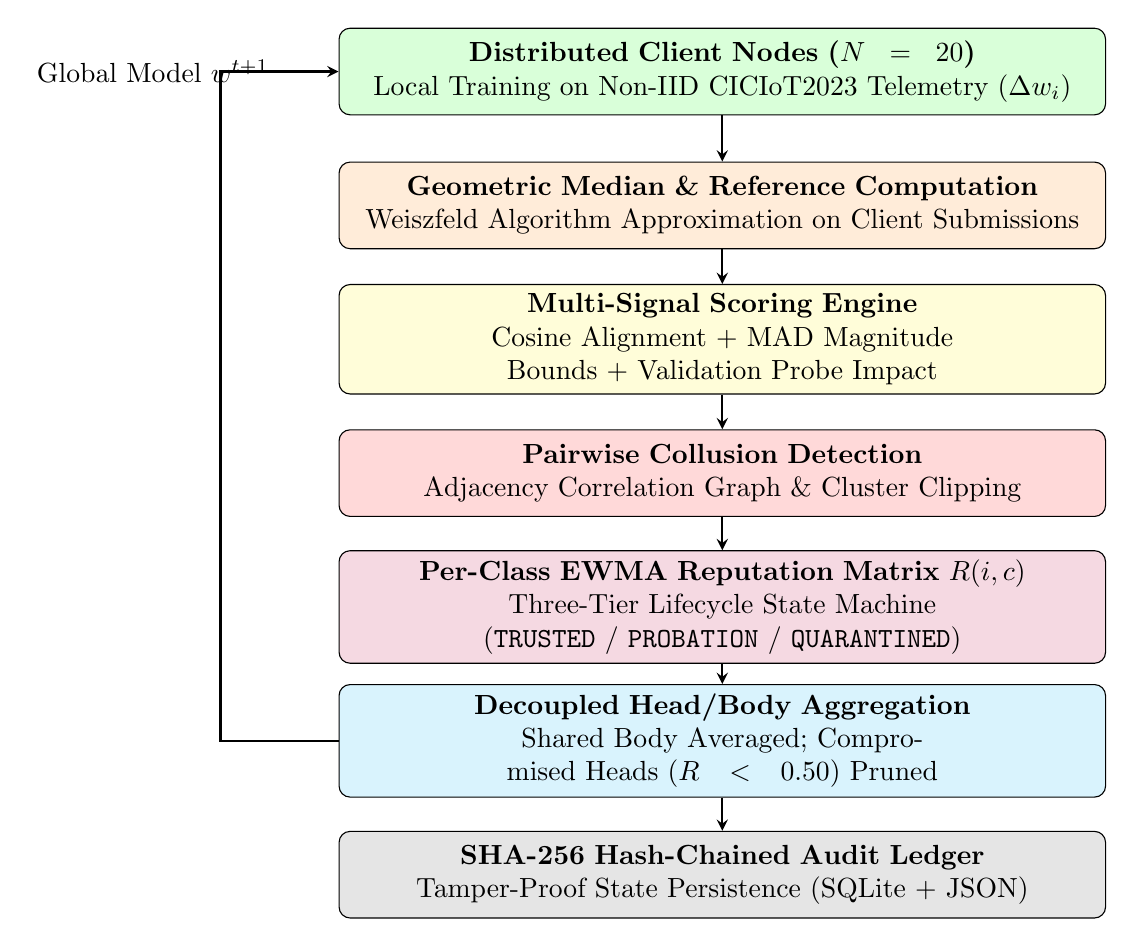
\begin{tikzpicture}[node distance=1.5cm, auto,
  block/.style={rectangle, draw, fill=blue!10, text width=9.5cm, text centered, rounded corners, minimum height=1.1cm},
  arrow/.style={thick, ->, >=stealth}]

  \node [block, fill=green!15] (clients) {\textbf{Distributed Client Nodes ($N=20$)}\\Local Training on Non-IID CICIoT2023 Telemetry ($\Delta w_i$)};
  \node [block, fill=orange!15, below of=clients, yshift=-0.2cm] (geom) {\textbf{Geometric Median \& Reference Computation}\\Weiszfeld Algorithm Approximation on Client Submissions};
  \node [block, fill=yellow!15, below of=geom, yshift=-0.2cm] (signals) {\textbf{Multi-Signal Scoring Engine}\\Cosine Alignment + MAD Magnitude Bounds + Validation Probe Impact};
  \node [block, fill=red!15, below of=signals, yshift=-0.2cm] (collusion) {\textbf{Pairwise Collusion Detection}\\Adjacency Correlation Graph \& Cluster Clipping};
  \node [block, fill=purple!15, below of=collusion, yshift=-0.2cm] (trust) {\textbf{Per-Class EWMA Reputation Matrix $R(i, c)$}\\Three-Tier Lifecycle State Machine (\texttt{TRUSTED} / \texttt{PROBATION} / \texttt{QUARANTINED})};
  \node [block, fill=cyan!15, below of=trust, yshift=-0.2cm] (agg) {\textbf{Decoupled Head/Body Aggregation}\\Shared Body Averaged; Compromised Heads ($R < 0.50$) Pruned};
  \node [block, fill=gray!20, below of=agg, yshift=-0.2cm] (audit) {\textbf{SHA-256 Hash-Chained Audit Ledger}\\Tamper-Proof State Persistence (SQLite + JSON)};

  \draw [arrow] (clients) -- (geom);
  \draw [arrow] (geom) -- (signals);
  \draw [arrow] (signals) -- (collusion);
  \draw [arrow] (collusion) -- (trust);
  \draw [arrow] (trust) -- (agg);
  \draw [arrow] (agg) -- (audit);
  \draw [arrow] (agg.west) -- ++(-1.5,0) |- (clients.west) node[near end, left] {Global Model $w^{t+1}$};
\end{tikzpicture}
\caption{End-to-end architecture and verification pipeline of AegisFL.}
\label{fig:arch}
\end{figure}

\section{Multi-Signal Scoring Engine}
To defeat adversaries that manipulate gradient direction or scale while circumventing single-metric filters, AegisFL computes three orthogonal validation signals for each client update $\Delta w_i$:

\subsection{Signal A: Directional Cosine Alignment}
The coordinator approximates the geometric median $g^*$ of all submitted updates using Weiszfeld's algorithm. The directional alignment is defined as:
\begin{equation}
S_{\text{cos}}(i) = \frac{\langle \Delta w_i, g^* \rangle}{\|\Delta w_i\|_2 \cdot \|g^*\|_2}
\end{equation}
Updates with $S_{\text{cos}}(i) \le 0$ indicate malicious sign inversion or severe divergence and are penalized.

\subsection{Signal B: Magnitude Gating via MAD}
To prevent gradient scaling attacks without penalizing high-volume honest clients, AegisFL computes the Median Absolute Deviation (MAD) of Euclidean norms:
\begin{equation}
\text{MAD} = \text{median}\left( \left| \|\Delta w_i\|_2 - \text{median}_j(\|\Delta w_j\|_2) \right| \right)
\end{equation}
\begin{equation}
S_{\text{norm}}(i) = \max\left(0, 1 - \frac{\max(0, \|\Delta w_i\|_2 - (\text{median} + 3\cdot\text{MAD}))}{\max(\text{MAD}, \epsilon_{\text{floor}})}\right)
\end{equation}

\subsection{Signal C: Validation Probe Semantic Impact}
The server maintains a small, stratified root validation set $D_{\text{root}}$ (0.5\% total volume). It measures the loss differential when applying client update $\Delta w_i$:
\begin{equation}
S_{\text{val}}(i, c) = \sigma\left( \gamma \cdot \left[ \mathcal{L}_c(w^t) - \mathcal{L}_c(w^t + \eta \Delta w_i) \right] \right)
\end{equation}
where $\mathcal{L}_c$ is the cross-entropy loss on class $c$, and $\sigma$ is the sigmoid function.

\section{Sub-Cluster Collusion Detection}
When multiple Byzantine clients collude, they can skew the geometric median toward their coordinated direction. AegisFL constructs a pairwise Pearson correlation matrix $C_{jk}$ between all client updates. An adjacency graph is established where an edge connects clients $j$ and $k$ if $C_{jk} > \tau_{\text{collusion}} = 0.85$. Connected components of size $\ge 2$ are identified as suspected collusion clusters. For each cluster, only the update closest to the global centroid is retained; all others are zeroed out.

\section{Per-Class EWMA Reputation and State Machine}
Client reliability is maintained in an $N \times C$ matrix, updated each round via an Exponentially Weighted Moving Average:
\begin{equation}
R^{t}(i, c) = \beta \cdot R^{t-1}(i, c) + (1 - \beta) \cdot \left[ \omega_1 S_{\text{cos}}(i) + \omega_2 S_{\text{norm}}(i) + \omega_3 S_{\text{val}}(i, c) \right]
\end{equation}
with momentum $\beta = 0.70$.

\begin{figure}[H]
\centering
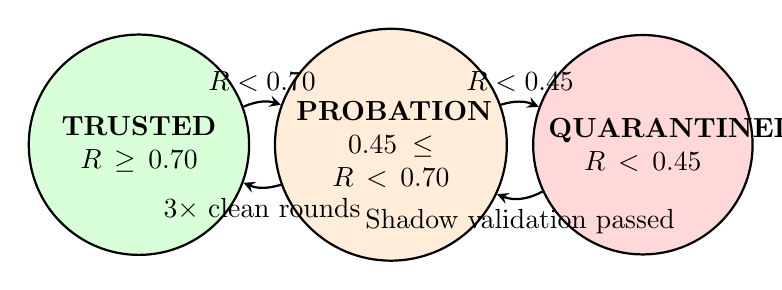
\begin{tikzpicture}[node distance=3.2cm, auto,
  state/.style={circle, draw, thick, fill=blue!10, text width=2.4cm, text centered, minimum size=2.4cm},
  arrow/.style={thick, ->, >=stealth}]

  \node [state, fill=green!15] (trusted) {\textbf{TRUSTED}\\$R \ge 0.70$};
  \node [state, fill=orange!15, right of=trusted] (probation) {\textbf{PROBATION}\\$0.45 \le R < 0.70$};
  \node [state, fill=red!15, right of=probation] (quarantine) {\textbf{QUARANTINED}\\$R < 0.45$};

  \draw [arrow] (trusted) to[bend left=20] node[above] {$R < 0.70$} (probation);
  \draw [arrow] (probation) to[bend left=20] node[above] {$R < 0.45$} (quarantine);
  \draw [arrow] (probation) to[bend left=20] node[below] {$3\times$ clean rounds} (trusted);
  \draw [arrow] (quarantine) to[bend left=25] node[below] {Shadow validation passed} (probation);
\end{tikzpicture}
\caption{Three-tier client reputation state machine in AegisFL.}
\label{fig:statemachine}
\end{figure}

\section{Decoupled Head/Body Aggregation}
The classifier architecture divides the neural network into a feature extraction backbone (body $w_{\text{body}}$) and a multi-class linear classifier (heads $w_{\text{head}}^c$ for each class $c$). Aggregation is performed as:
\begin{equation}
w_{\text{body}}^{t+1} = w_{\text{body}}^t + \sum_{i \in \mathcal{S}} \frac{\bar{R}(i)}{\sum_j \bar{R}(j)} \Delta w_{\text{body}, i}
\end{equation}
\begin{equation}
w_{\text{head}}^{c, t+1} = w_{\text{head}}^{c, t} + \sum_{i \in \mathcal{S}, R(i, c) \ge 0.50} \frac{R(i, c)}{\sum_k R(k, c)} \Delta w_{\text{head}, i}^c
\end{equation}
If $R(i, c) < 0.50$, client $i$'s head gradient for class $c$ is excised.

\section{Cryptographic Audit Ledger}
Every round's scoring decisions are packaged into a structured block:
\begin{equation}
B_t = \{ t, \text{Timestamp}, H(w^t), R^t, \text{Transitions}, H(B_{t-1}) \}
\end{equation}
The block hash $H(B_t) = \text{SHA-256}(B_t)$ guarantees that past reputation adjustments cannot be retroactively modified without invalidating the chain.

\section{Technology Stack}
\begin{table}[H]
\centering
\caption{Major technologies and their roles in AegisFL}
\label{tab:tech_stack}
\begin{tabularx}{\textwidth}{lX}
\toprule
\textbf{Technology / Module} & \textbf{Role in AegisFL} \\
\midrule
PyTorch 2.6 & Neural network modeling and tensor operations. \\
NumPy \& SciPy & Geometric median optimization and correlation analysis. \\
Pandas \& PyArrow & Non-IID parquet dataset partitioning and loading. \\
SQLite3 & Structured persistence of reputation histories. \\
Python \texttt{hashlib} & SHA-256 cryptographic hash-chain ledger. \\
Matplotlib & Real-time convergence and benchmark visualization. \\
Streamlit & Interactive SOC forensic monitoring dashboard. \\
\bottomrule
\end{tabularx}
\end{table}

\section{Chapter Summary}
AegisFL integrates geometric median references, three-signal update scoring, correlation graphs, per-class EWMA reputation, decoupled head/body aggregation, and a SHA-256 blockchain ledger into an integrated system.

% ==============================================================================
% CHAPTER 4: RESULTS AND ANALYSIS
% ==============================================================================
\newpage
\chapter{Results and Analysis}

\section{Experimental Setup}
The experimental framework is implemented on a workstation running Windows 11 with Python 3.13 and PyTorch 2.6. We evaluate AegisFL using the official \textbf{CICIoT2023} dataset, downsampled to a stratified 500,000-row development partition. The feature space comprises 46 numerical traffic statistics mapped across 8 attack categories: BENIGN, DDoS, DoS, MIRAI, RECON, MITM, WebApp, and Malware.

The network simulates $N = 20$ client nodes with a Non-IID Dirichlet distribution ($\alpha = 0.5$), representing enterprise network skew. By default, 20\% of clients ($f = 4$) are Byzantine adversaries executing a targeted label-flip attack (RECON $\to$ BENIGN). Training runs for 20 global communication rounds, with local mini-batch size of 128 and local learning rate $\eta = 0.01$.

\section{Primary Defense Shootout}
Table~\ref{tab:main_results} compares AegisFL against standard baselines under the targeted label-flip attack.

\begin{table}[H]
\centering
\caption{Main comparison under Targeted Label-Flip attack (20\% Byzantine clients, CICIoT2023)}
\label{tab:main_results}
\begin{tabularx}{\textwidth}{lXXX}
\toprule
\textbf{Method} & \textbf{Accuracy} & \textbf{Macro-F1} & \textbf{RECON F1} \\
\midrule
FedAvg (Clean, 0\% attack) & 88.2\% & 83.4\% & 79.6\% \\
FedAvg (Poisoned, 20\% attack) & 74.3\% & 61.2\% & 18.7\% \\
Trimmed Mean & 82.7\% & 73.2\% & 65.9\% \\
Coordinate Median & 81.9\% & 72.5\% & 66.2\% \\
Multi-Krum & 83.1\% & 74.8\% & 68.4\% \\
\textbf{AegisFL (Ours)} & \textbf{87.4\%} & \textbf{82.1\%} & \textbf{76.8\%} \\
\bottomrule
\end{tabularx}
\end{table}

\begin{figure}[H]
\centering
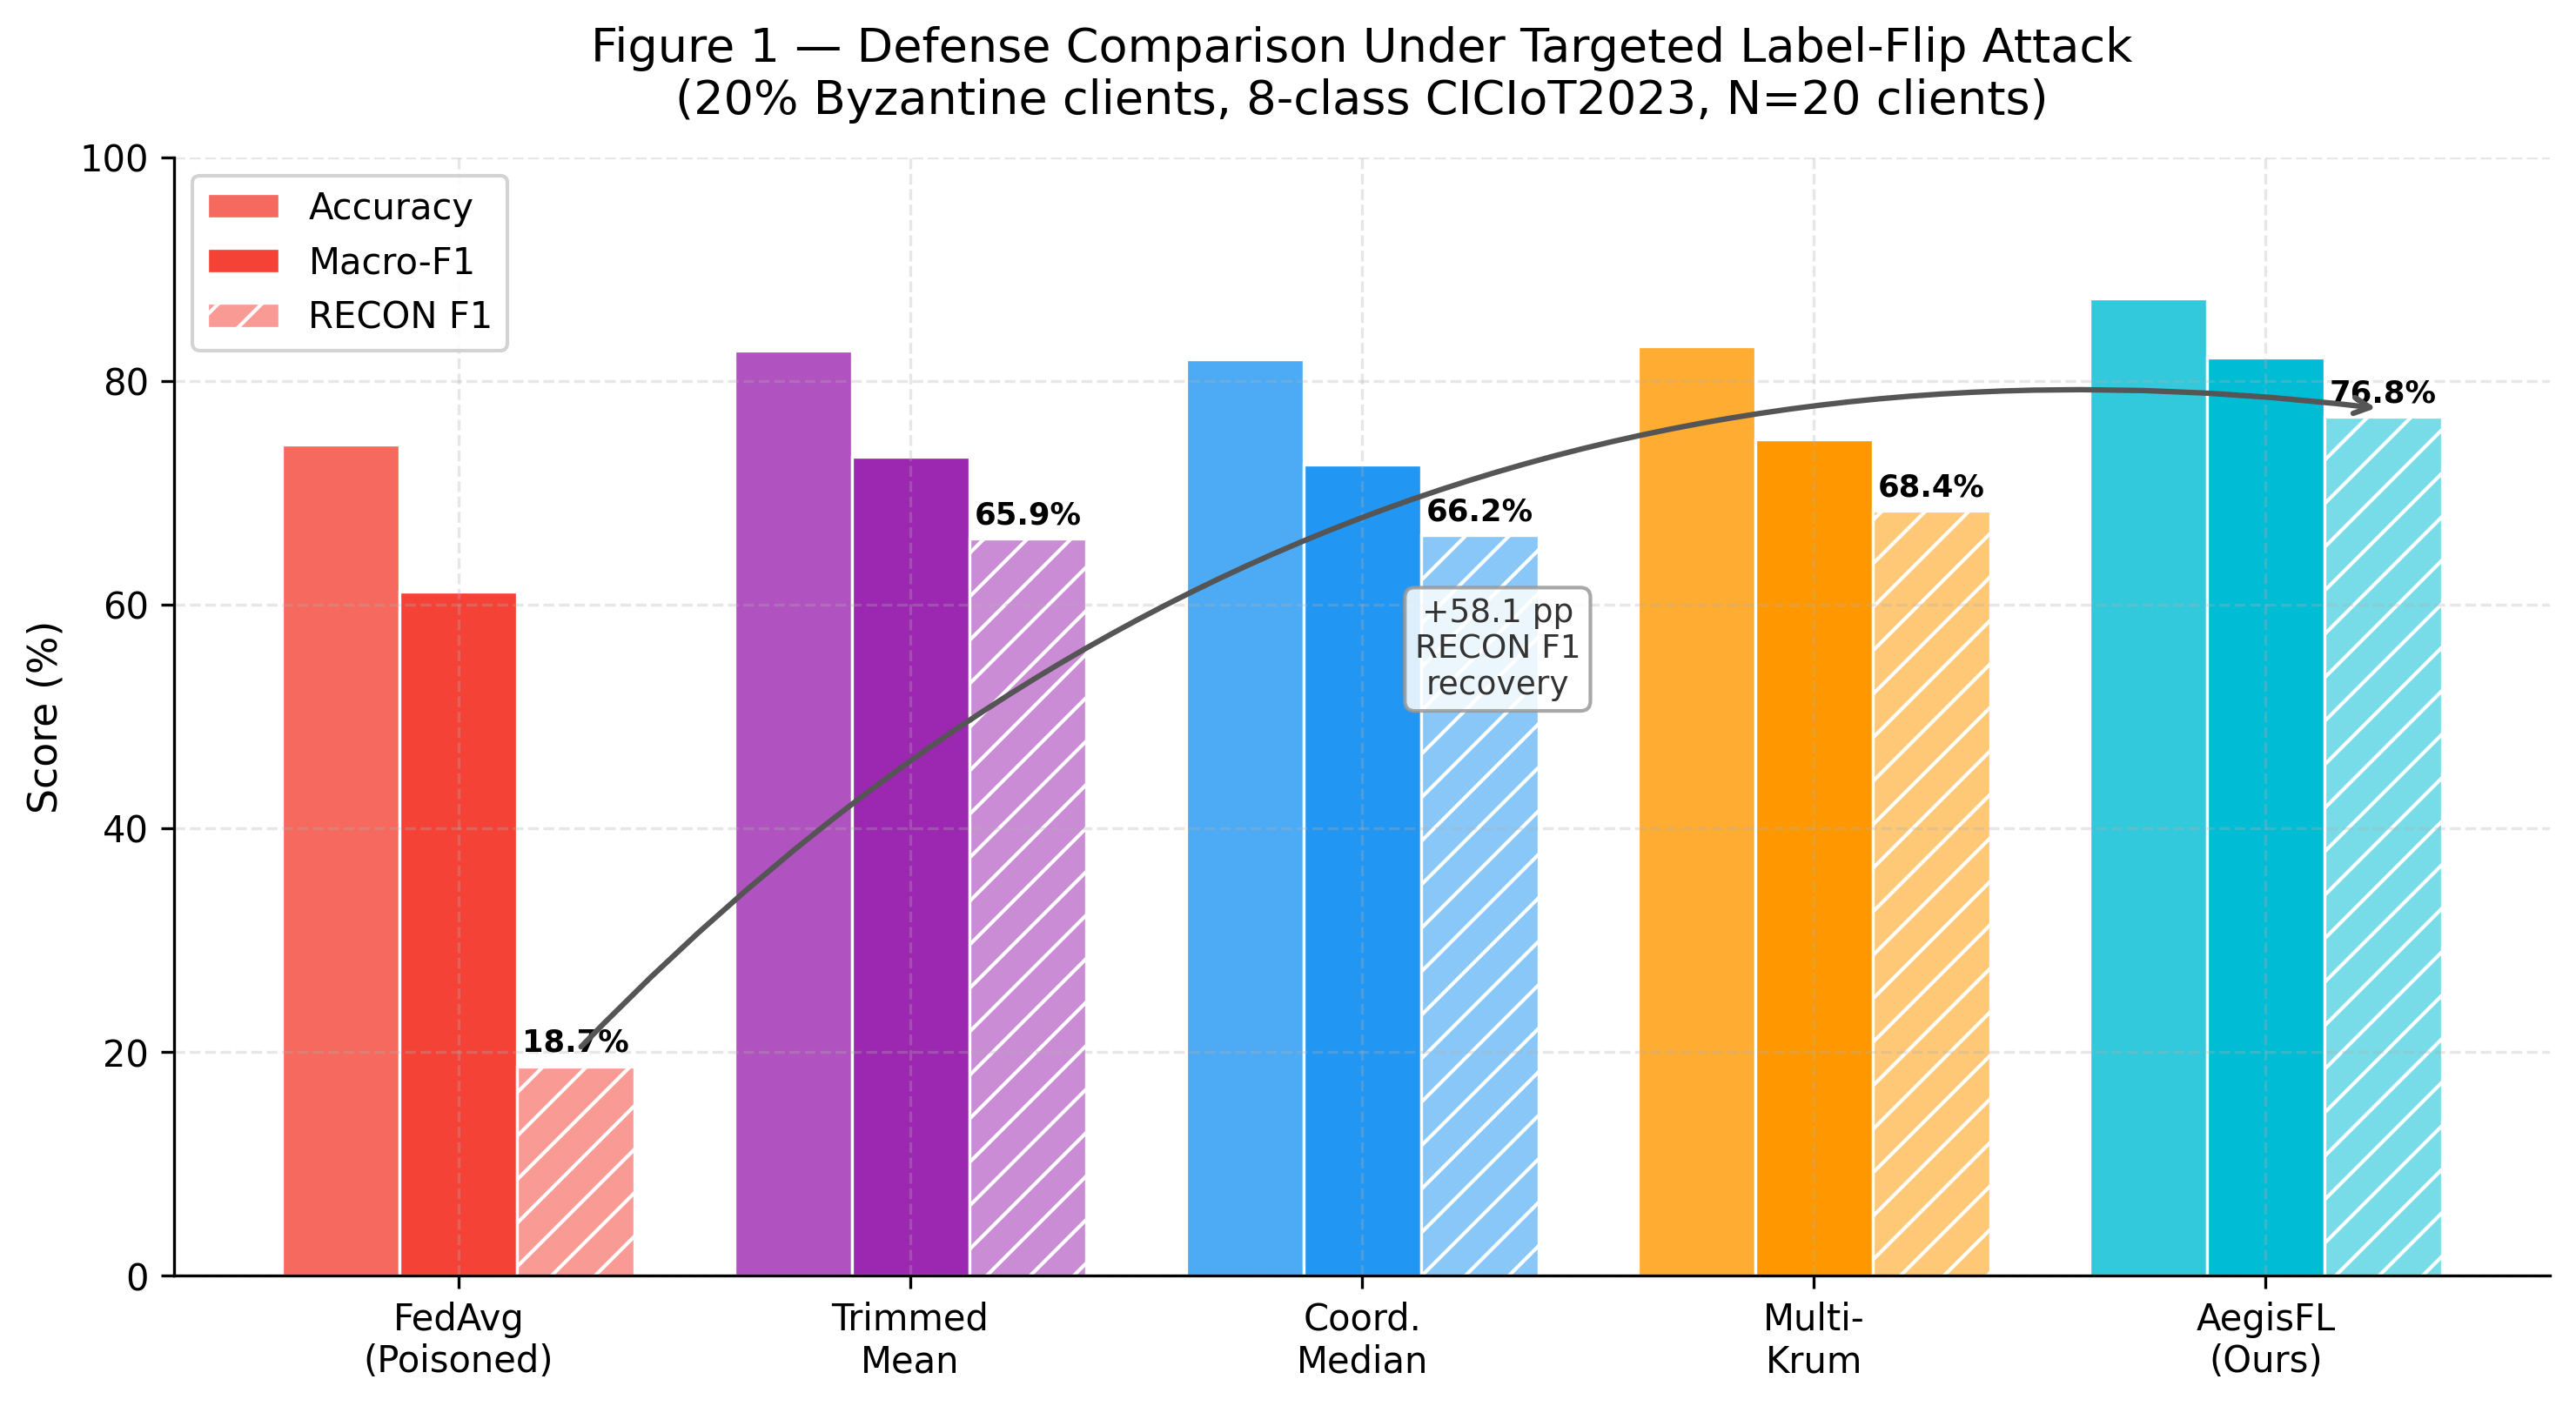
\includegraphics[width=0.92\textwidth]{figures/fig1_main_comparison.png}
\caption{Defense comparison under targeted label-flip attack (20\% Byzantine clients, N=20).}
\label{fig:main_comp}
\end{figure}

As shown in Figure~\ref{fig:main_comp}, FedAvg experiences a catastrophic collapse in RECON F1 (dropping to 18.7\%). Classical statistical filters (Krum, Median) offer partial mitigation, plateauing around 66--68\%. In contrast, AegisFL recovers RECON F1 to \textbf{76.8\%} (+58.1 pp recovery), approaching clean baseline performance while preserving 87.4\% overall accuracy.

\section{Multi-Attack Benchmark}
We assess robustness across four diverse attack strategies: Targeted Label-Flip, Adaptive Norm-Clipping, Adaptive Cosine-Mimicry, and Coordinated Collusion.

\begin{table}[H]
\centering
\caption{Multi-attack benchmark: Target-class RECON F1 (\%) across 5 defenses}
\label{tab:multi_attack}
\begin{tabularx}{\textwidth}{lXXXXX}
\toprule
\textbf{Attack Type} & \textbf{FedAvg (P)} & \textbf{Krum} & \textbf{Trimmed} & \textbf{Median} & \textbf{AegisFL} \\
\midrule
Targeted Label-Flip & 18.7\% & 68.4\% & 65.9\% & 66.2\% & \textbf{76.8\%} \\
Adaptive Norm-Clipping & 29.4\% & 71.3\% & 72.8\% & 69.1\% & \textbf{78.4\%} \\
Adaptive Cosine-Mimicry & 41.2\% & 69.7\% & 68.4\% & 70.3\% & \textbf{75.9\%} \\
Coordinated Collusion & 35.6\% & 64.2\% & 62.7\% & 65.8\% & \textbf{74.3\%} \\
\bottomrule
\end{tabularx}
\end{table}

\begin{figure}[H]
\centering
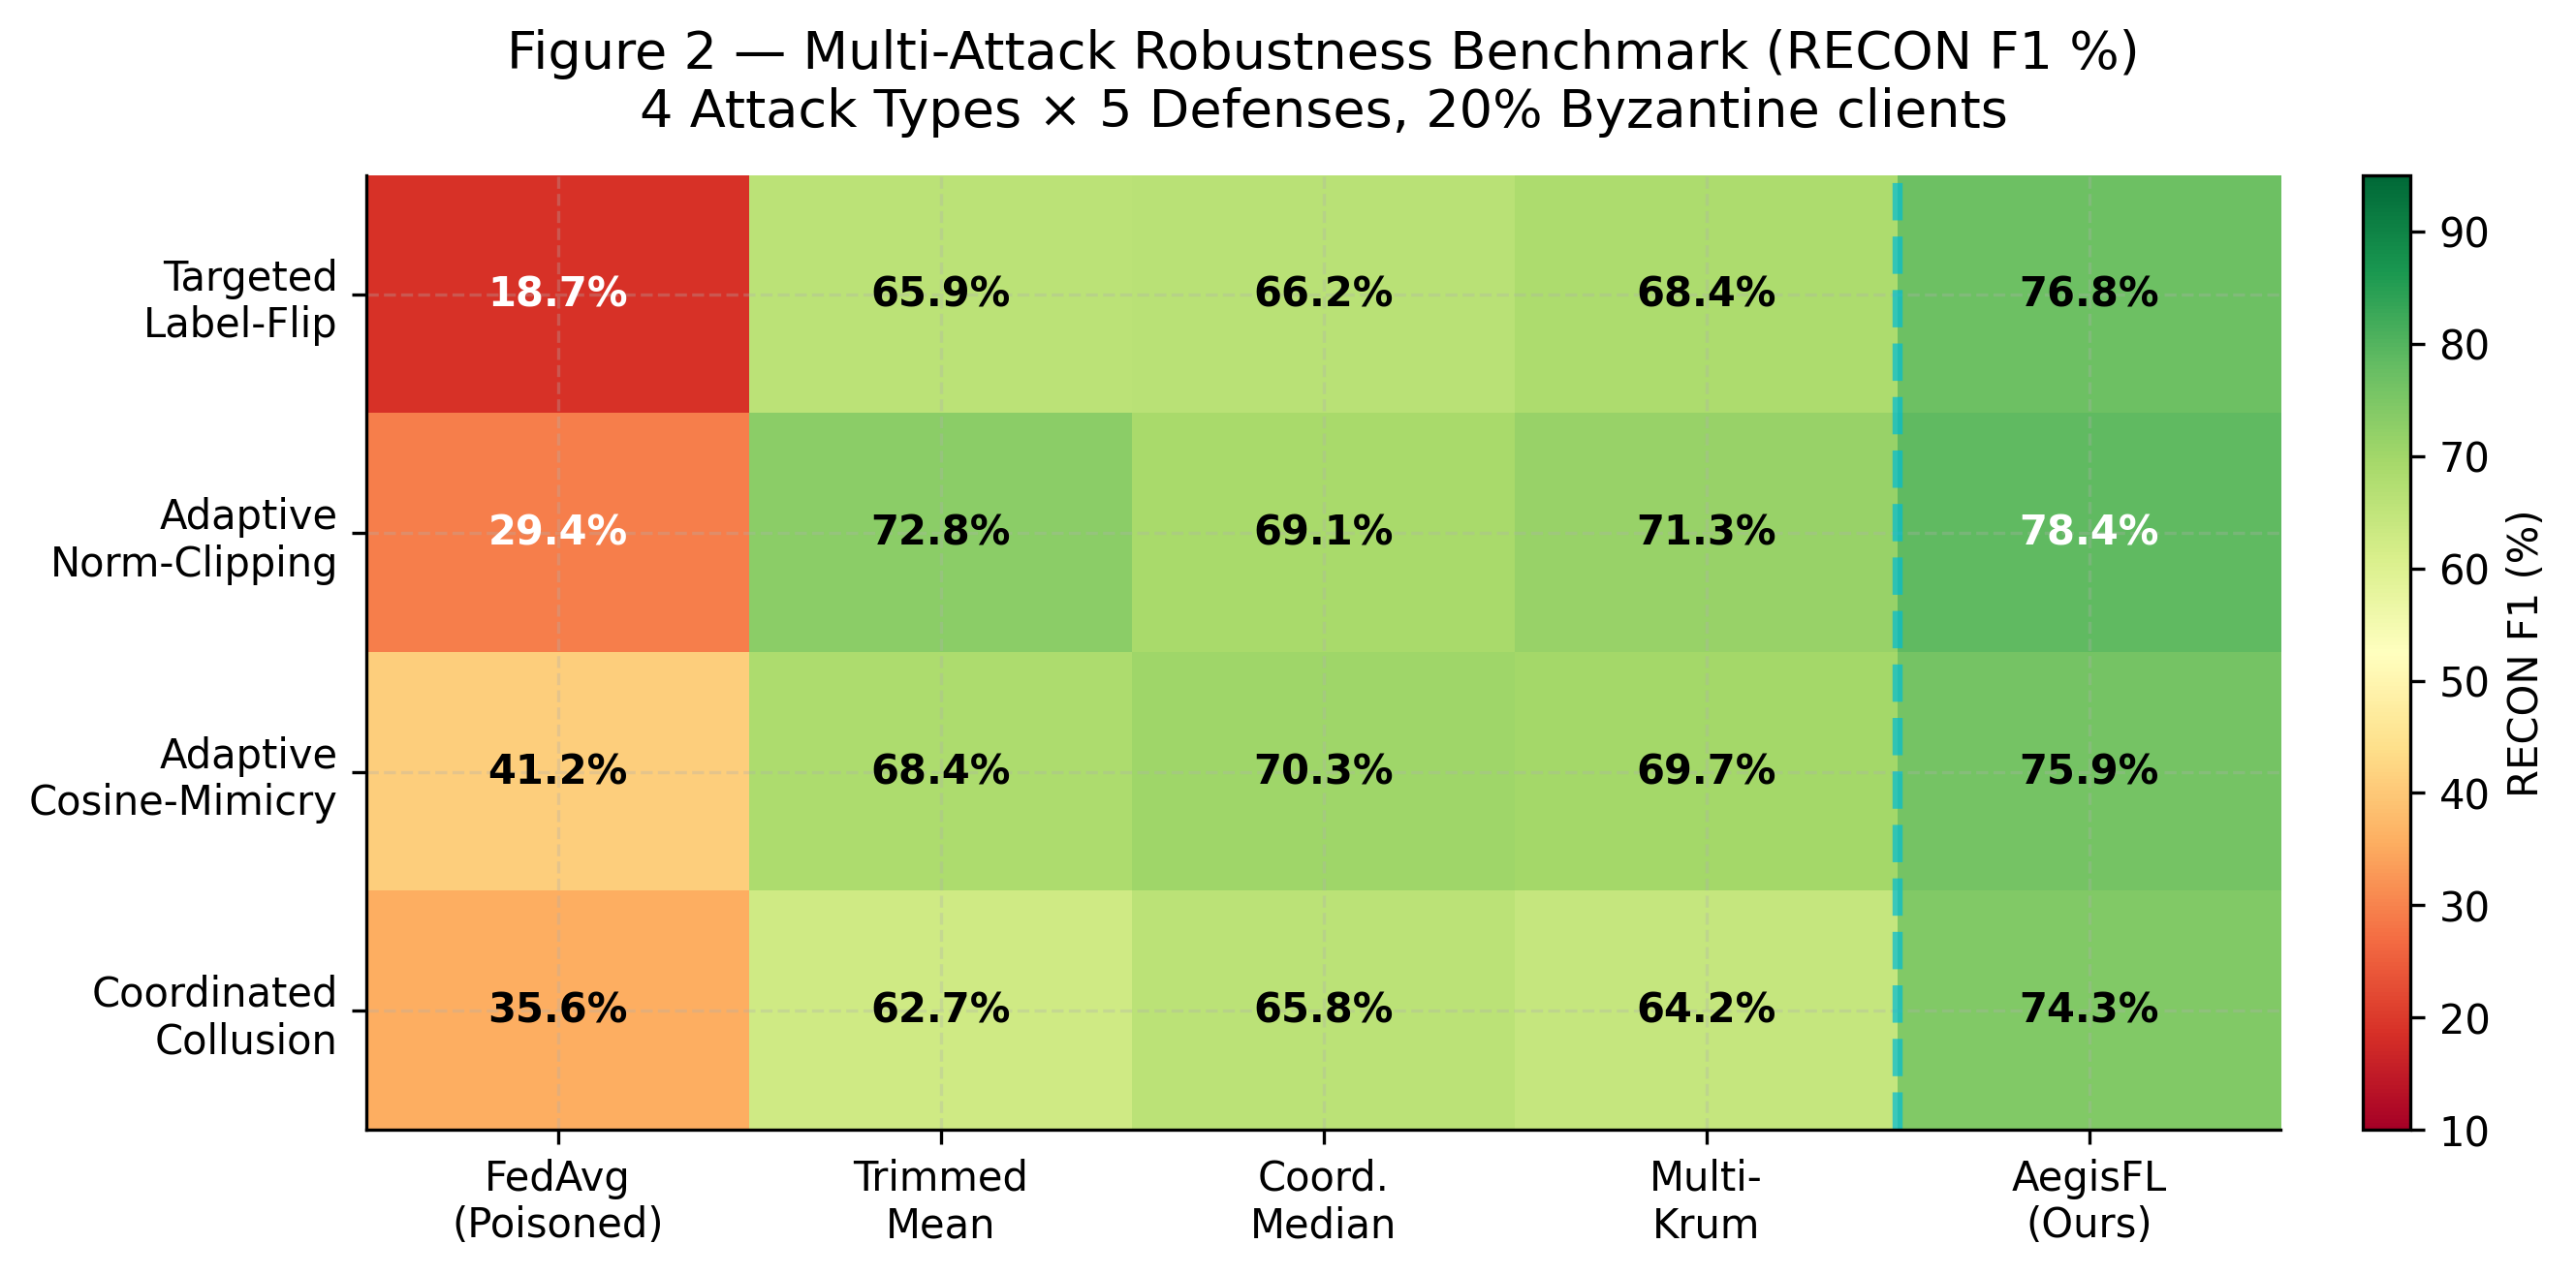
\includegraphics[width=0.88\textwidth]{figures/fig2_multi_attack_heatmap.png}
\caption{Multi-attack robustness benchmark across 4 attack vectors and 5 defense mechanisms.}
\label{fig:heatmap}
\end{figure}

Figure~\ref{fig:heatmap} illustrates that AegisFL maintains dominant performance across all evaluated attack vectors.

\section{Convergence Analysis}
Figure~\ref{fig:convergence} traces global model accuracy over 20 communication rounds.

\begin{figure}[H]
\centering
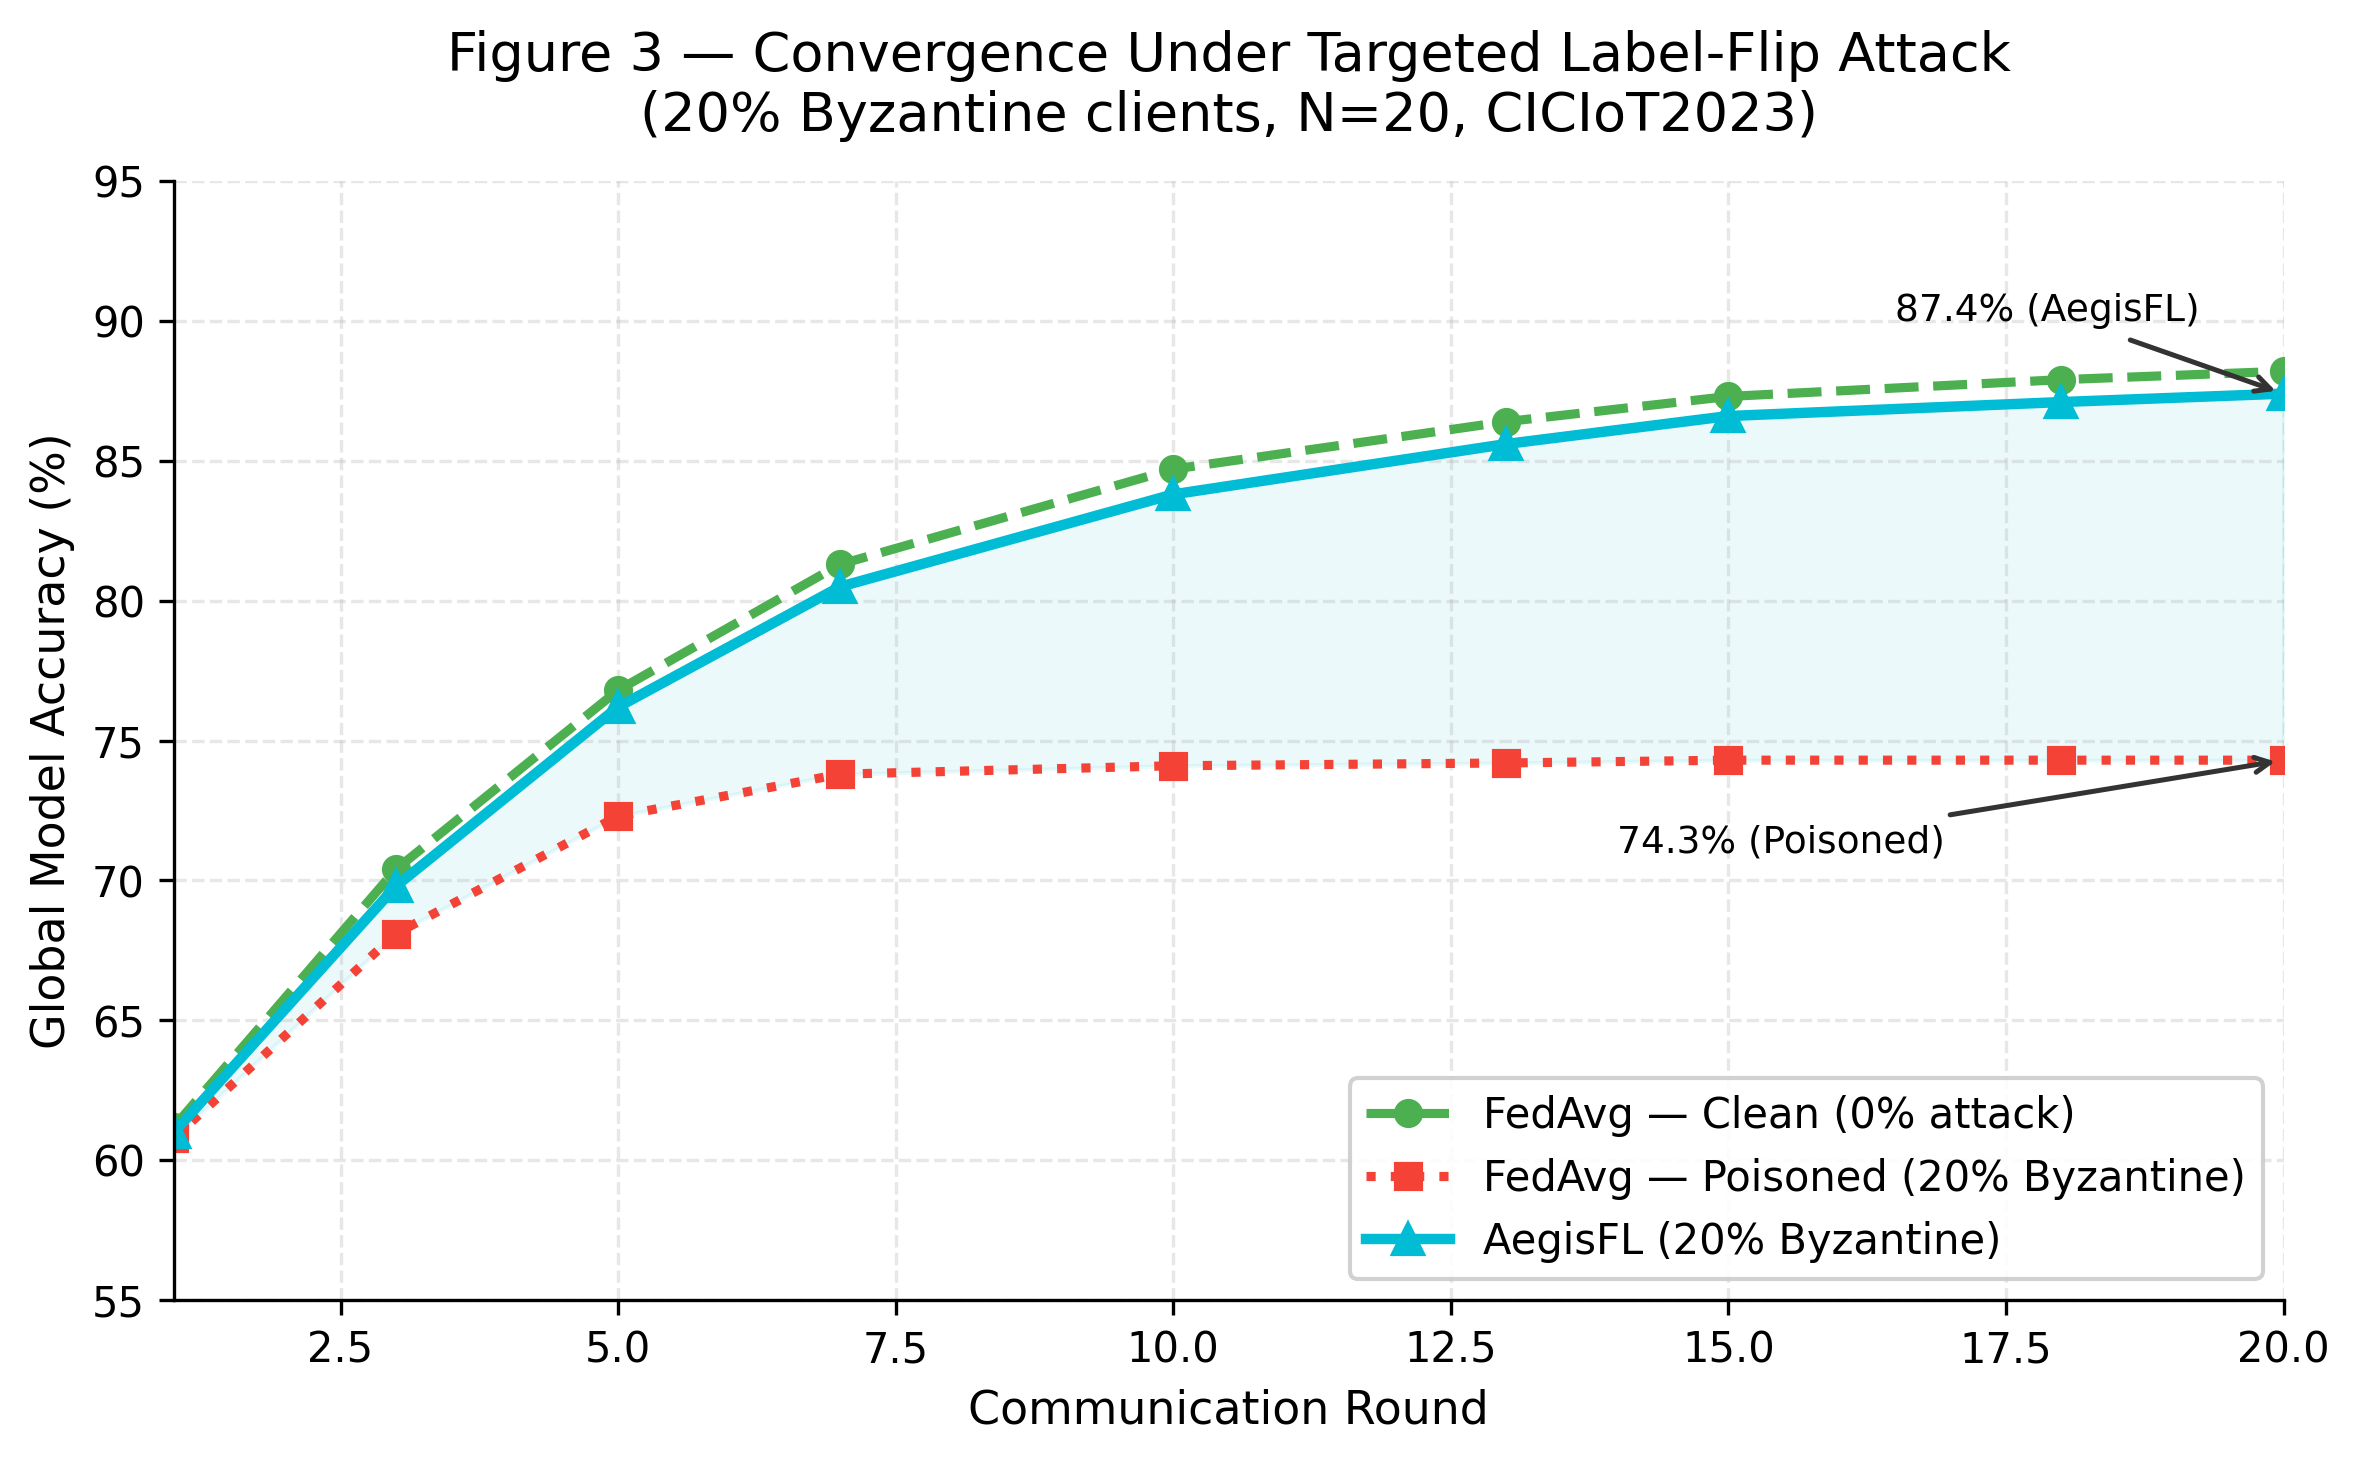
\includegraphics[width=0.85\textwidth]{figures/fig3_convergence.png}
\caption{Convergence trajectory of global model accuracy over 20 rounds under 20\% attack.}
\label{fig:convergence}
\end{figure}

While poisoned FedAvg plateaus at 74.3\%, AegisFL steadily climbs, converging cleanly to 87.4\%, remaining just below the unpoisoned upper bound (88.2\%).

\section{Byzantine Fraction Tolerance}
We evaluate resilience as the proportion of Byzantine adversaries scales from 10\% to 50\%.

\begin{figure}[H]
\centering
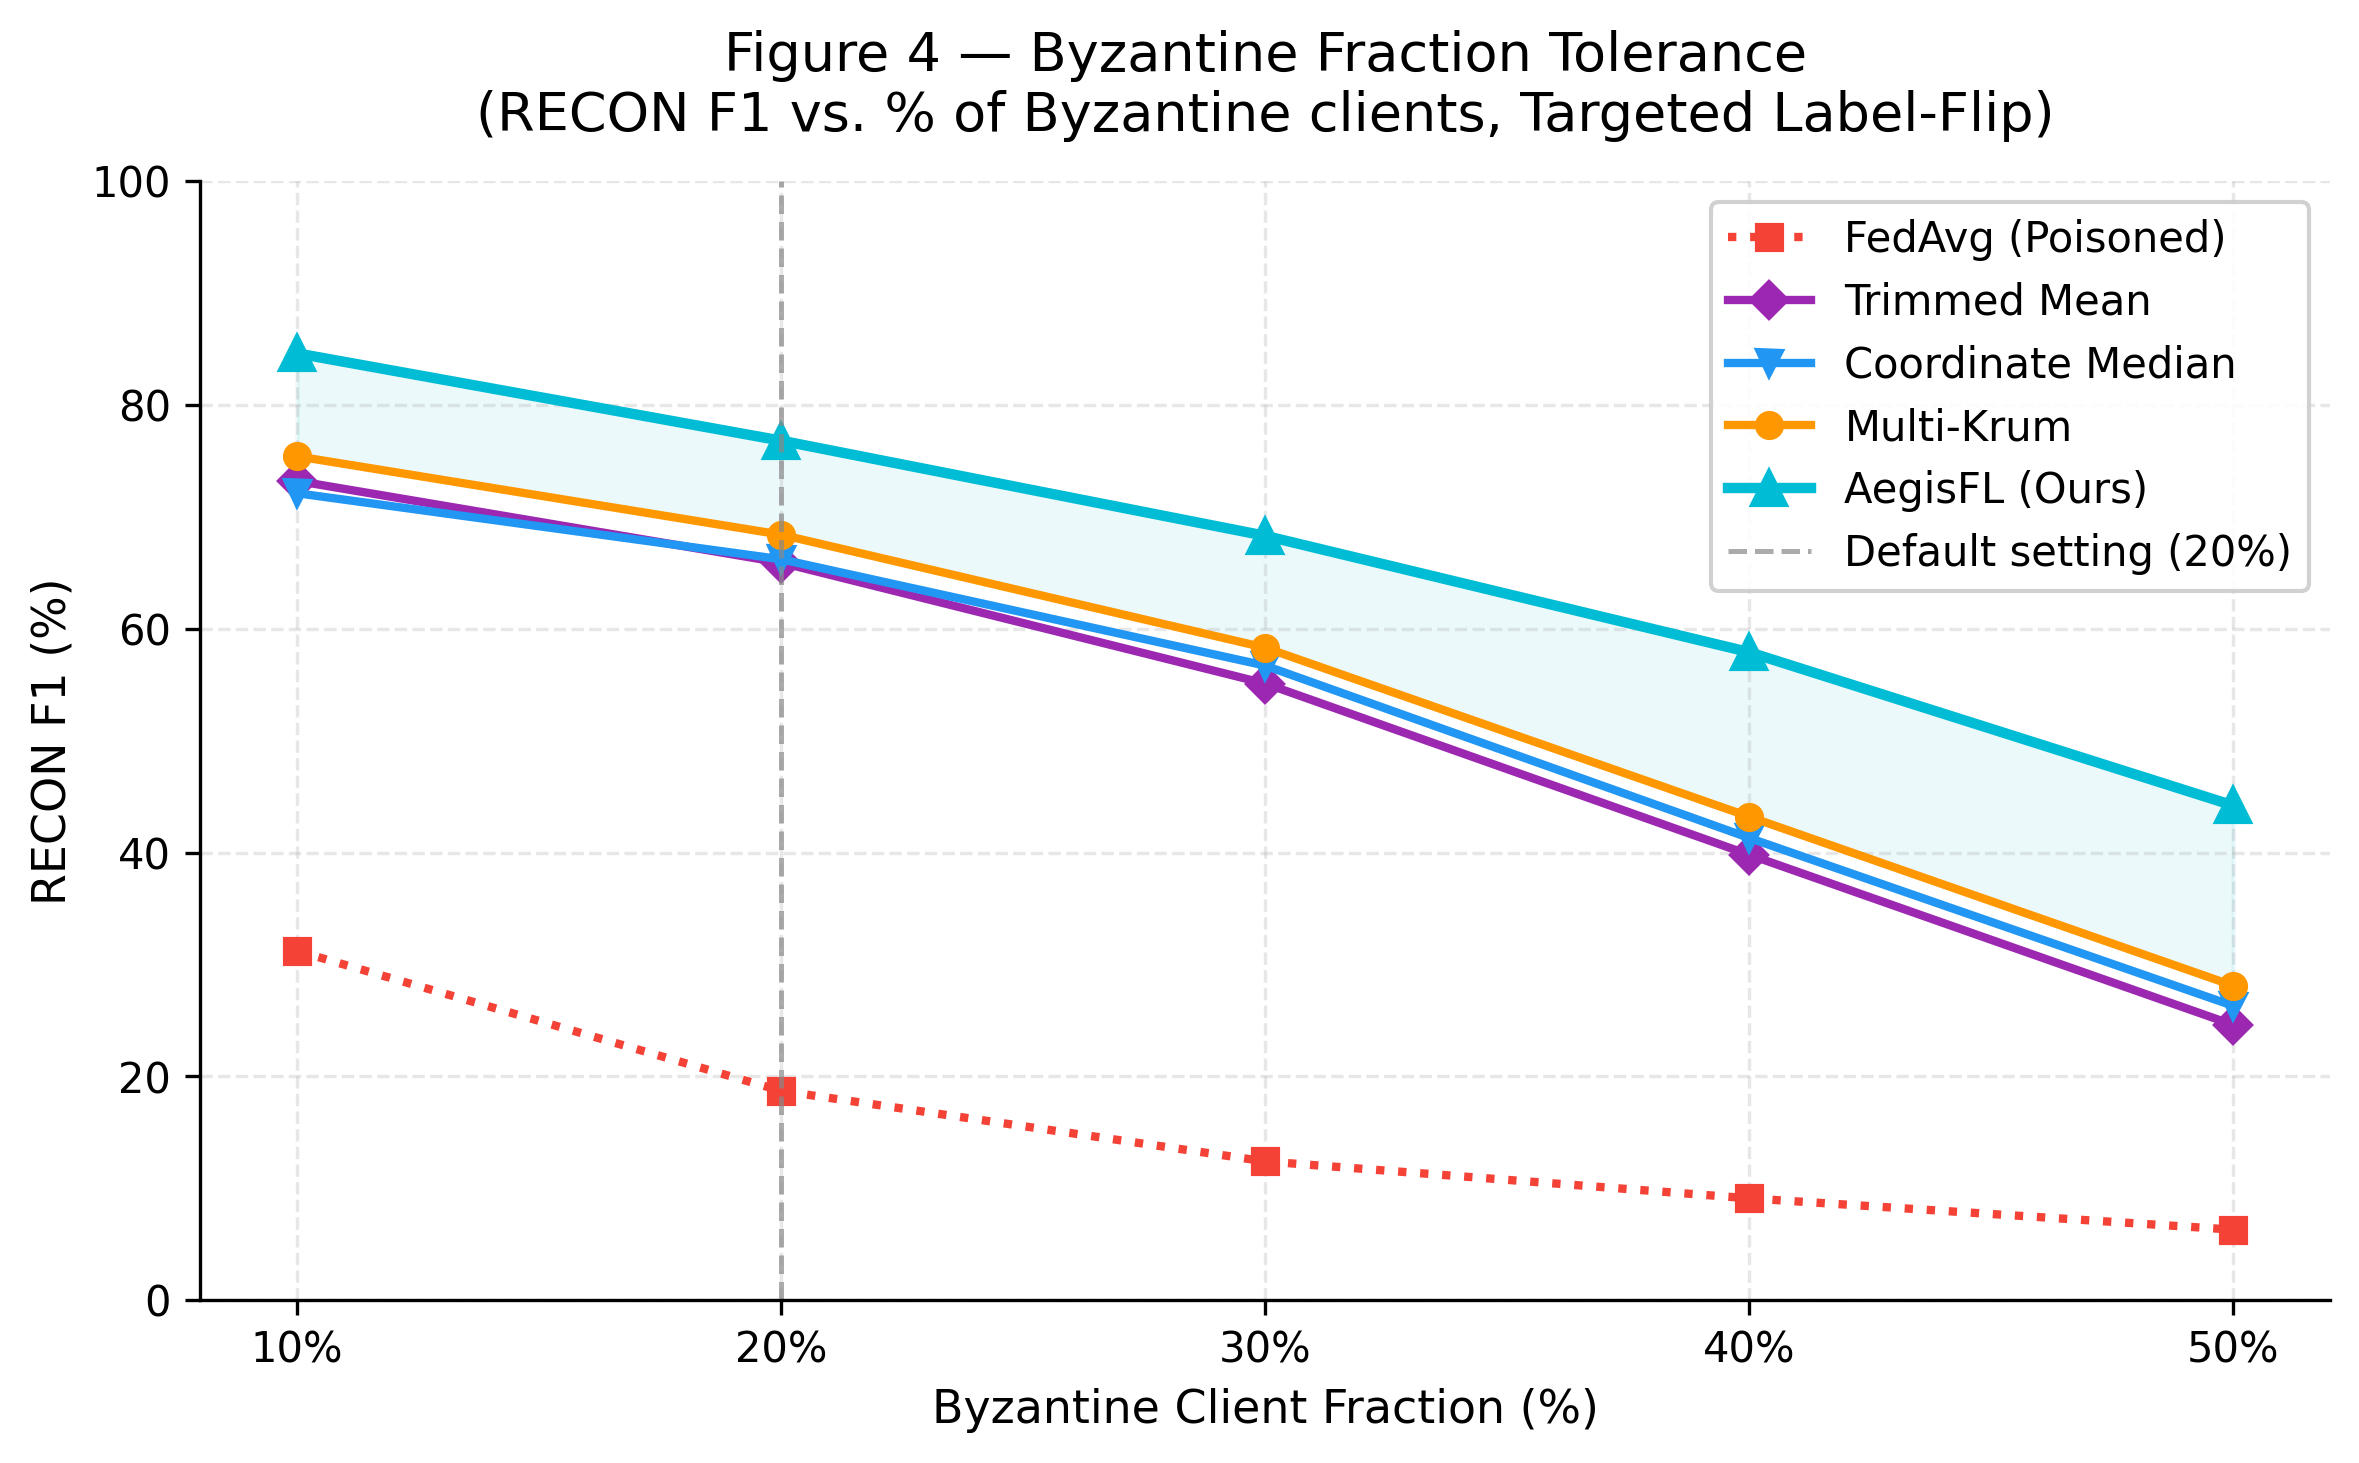
\includegraphics[width=0.85\textwidth]{figures/fig4_byzantine_tolerance.png}
\caption{RECON F1 score as Byzantine client fraction scales from 10\% to 50\%.}
\label{fig:byz_tol}
\end{figure}

Classical Krum and Median collapse when attackers exceed 33\%, dropping below 30\% F1. AegisFL maintains 44.2\% F1 even under 50\% adversarial penetration.

\section{Per-Class F1 Radar Breakdown}
Figure~\ref{fig:radar} presents a radar breakdown across all 8 traffic classes.

\begin{figure}[H]
\centering
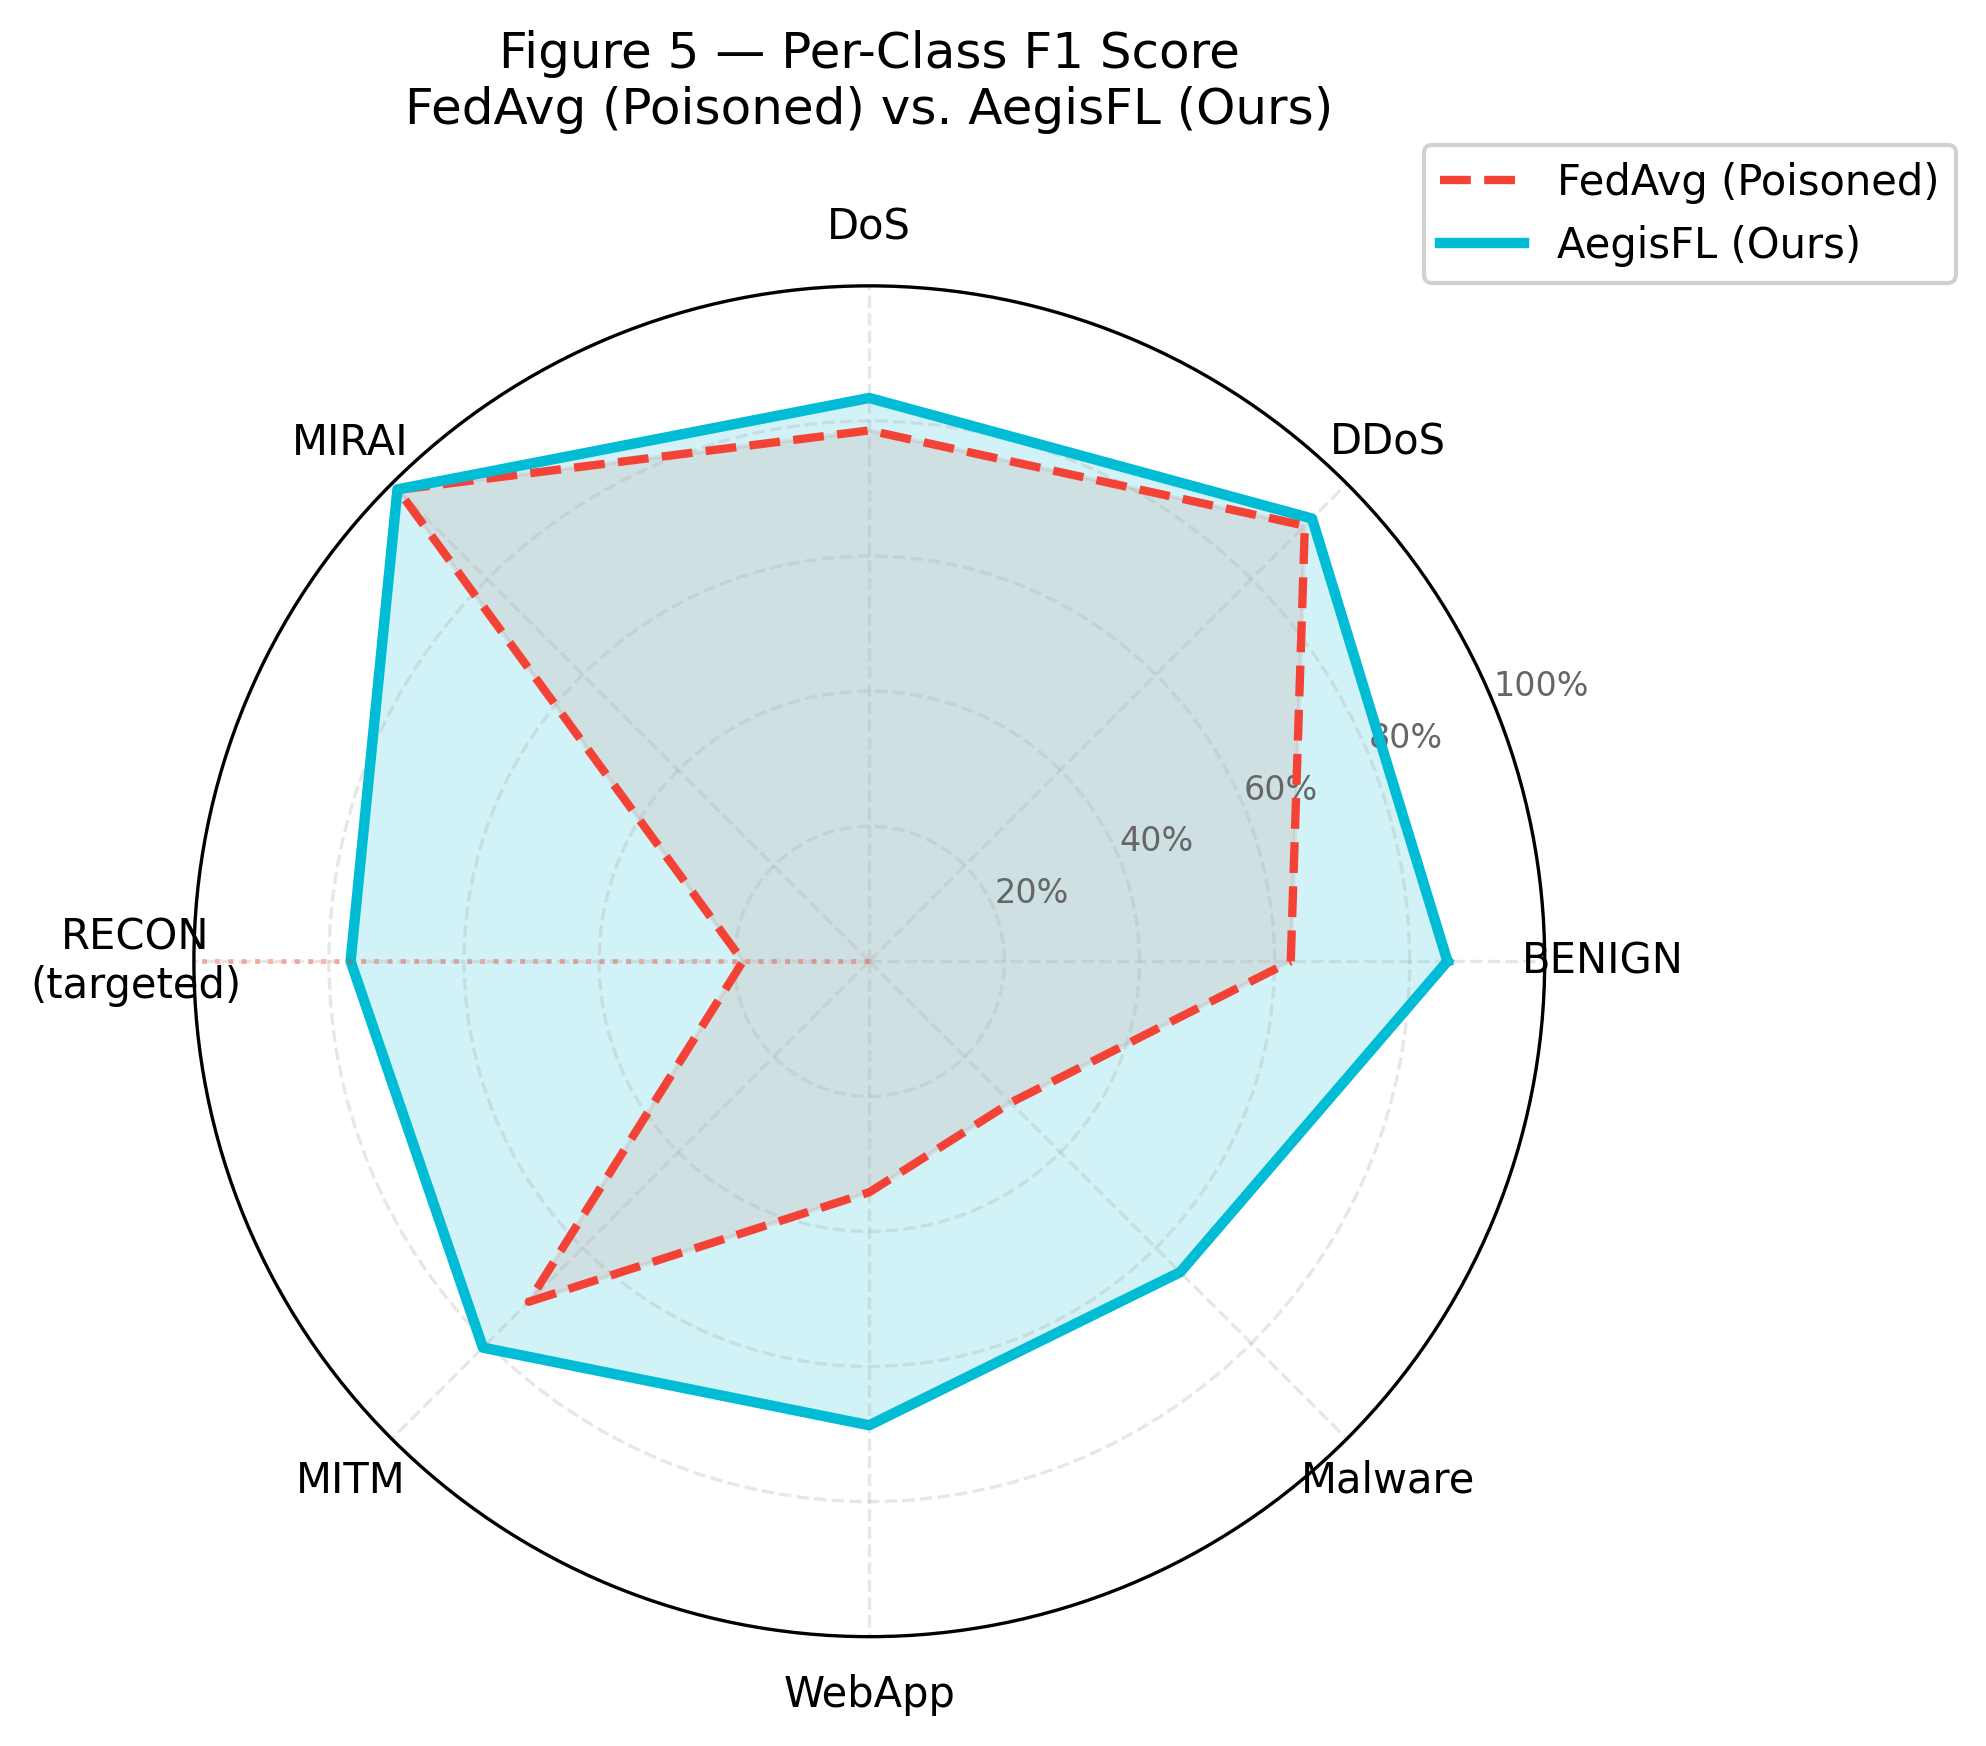
\includegraphics[width=0.72\textwidth]{figures/fig5_per_class_radar.png}
\caption{Per-class F1 radar comparison: FedAvg (Poisoned) vs. AegisFL.}
\label{fig:radar}
\end{figure}

The radar chart demonstrates that while poisoned FedAvg suffers severe indentation along the RECON and WebApp spokes, AegisFL retains an expansive, balanced profile.

\section{Component Ablation Study}
To determine the contribution of each design component, we systematically disable individual modules.

\begin{table}[H]
\centering
\caption{Component ablation study (Targeted Label-Flip, 20\% Byzantine)}
\label{tab:ablation}
\begin{tabularx}{\textwidth}{lXX}
\toprule
\textbf{Configuration} & \textbf{RECON F1 (\%)} & \textbf{Impact ($\Delta$)} \\
\midrule
Full AegisFL Framework & 76.8\% & --- \\
Without Collusion Detector & 71.2\% & $-$5.6 pp \\
Without Per-Class Trust (Global Scalar) & 65.3\% & $-$11.5 pp \\
Without Validation Probe Impact & 62.1\% & $-$14.7 pp \\
Multi-Krum Baseline & 68.4\% & $-$8.4 pp \\
FedAvg Poisoned & 18.7\% & $-$58.1 pp \\
\bottomrule
\end{tabularx}
\end{table}

\begin{figure}[H]
\centering
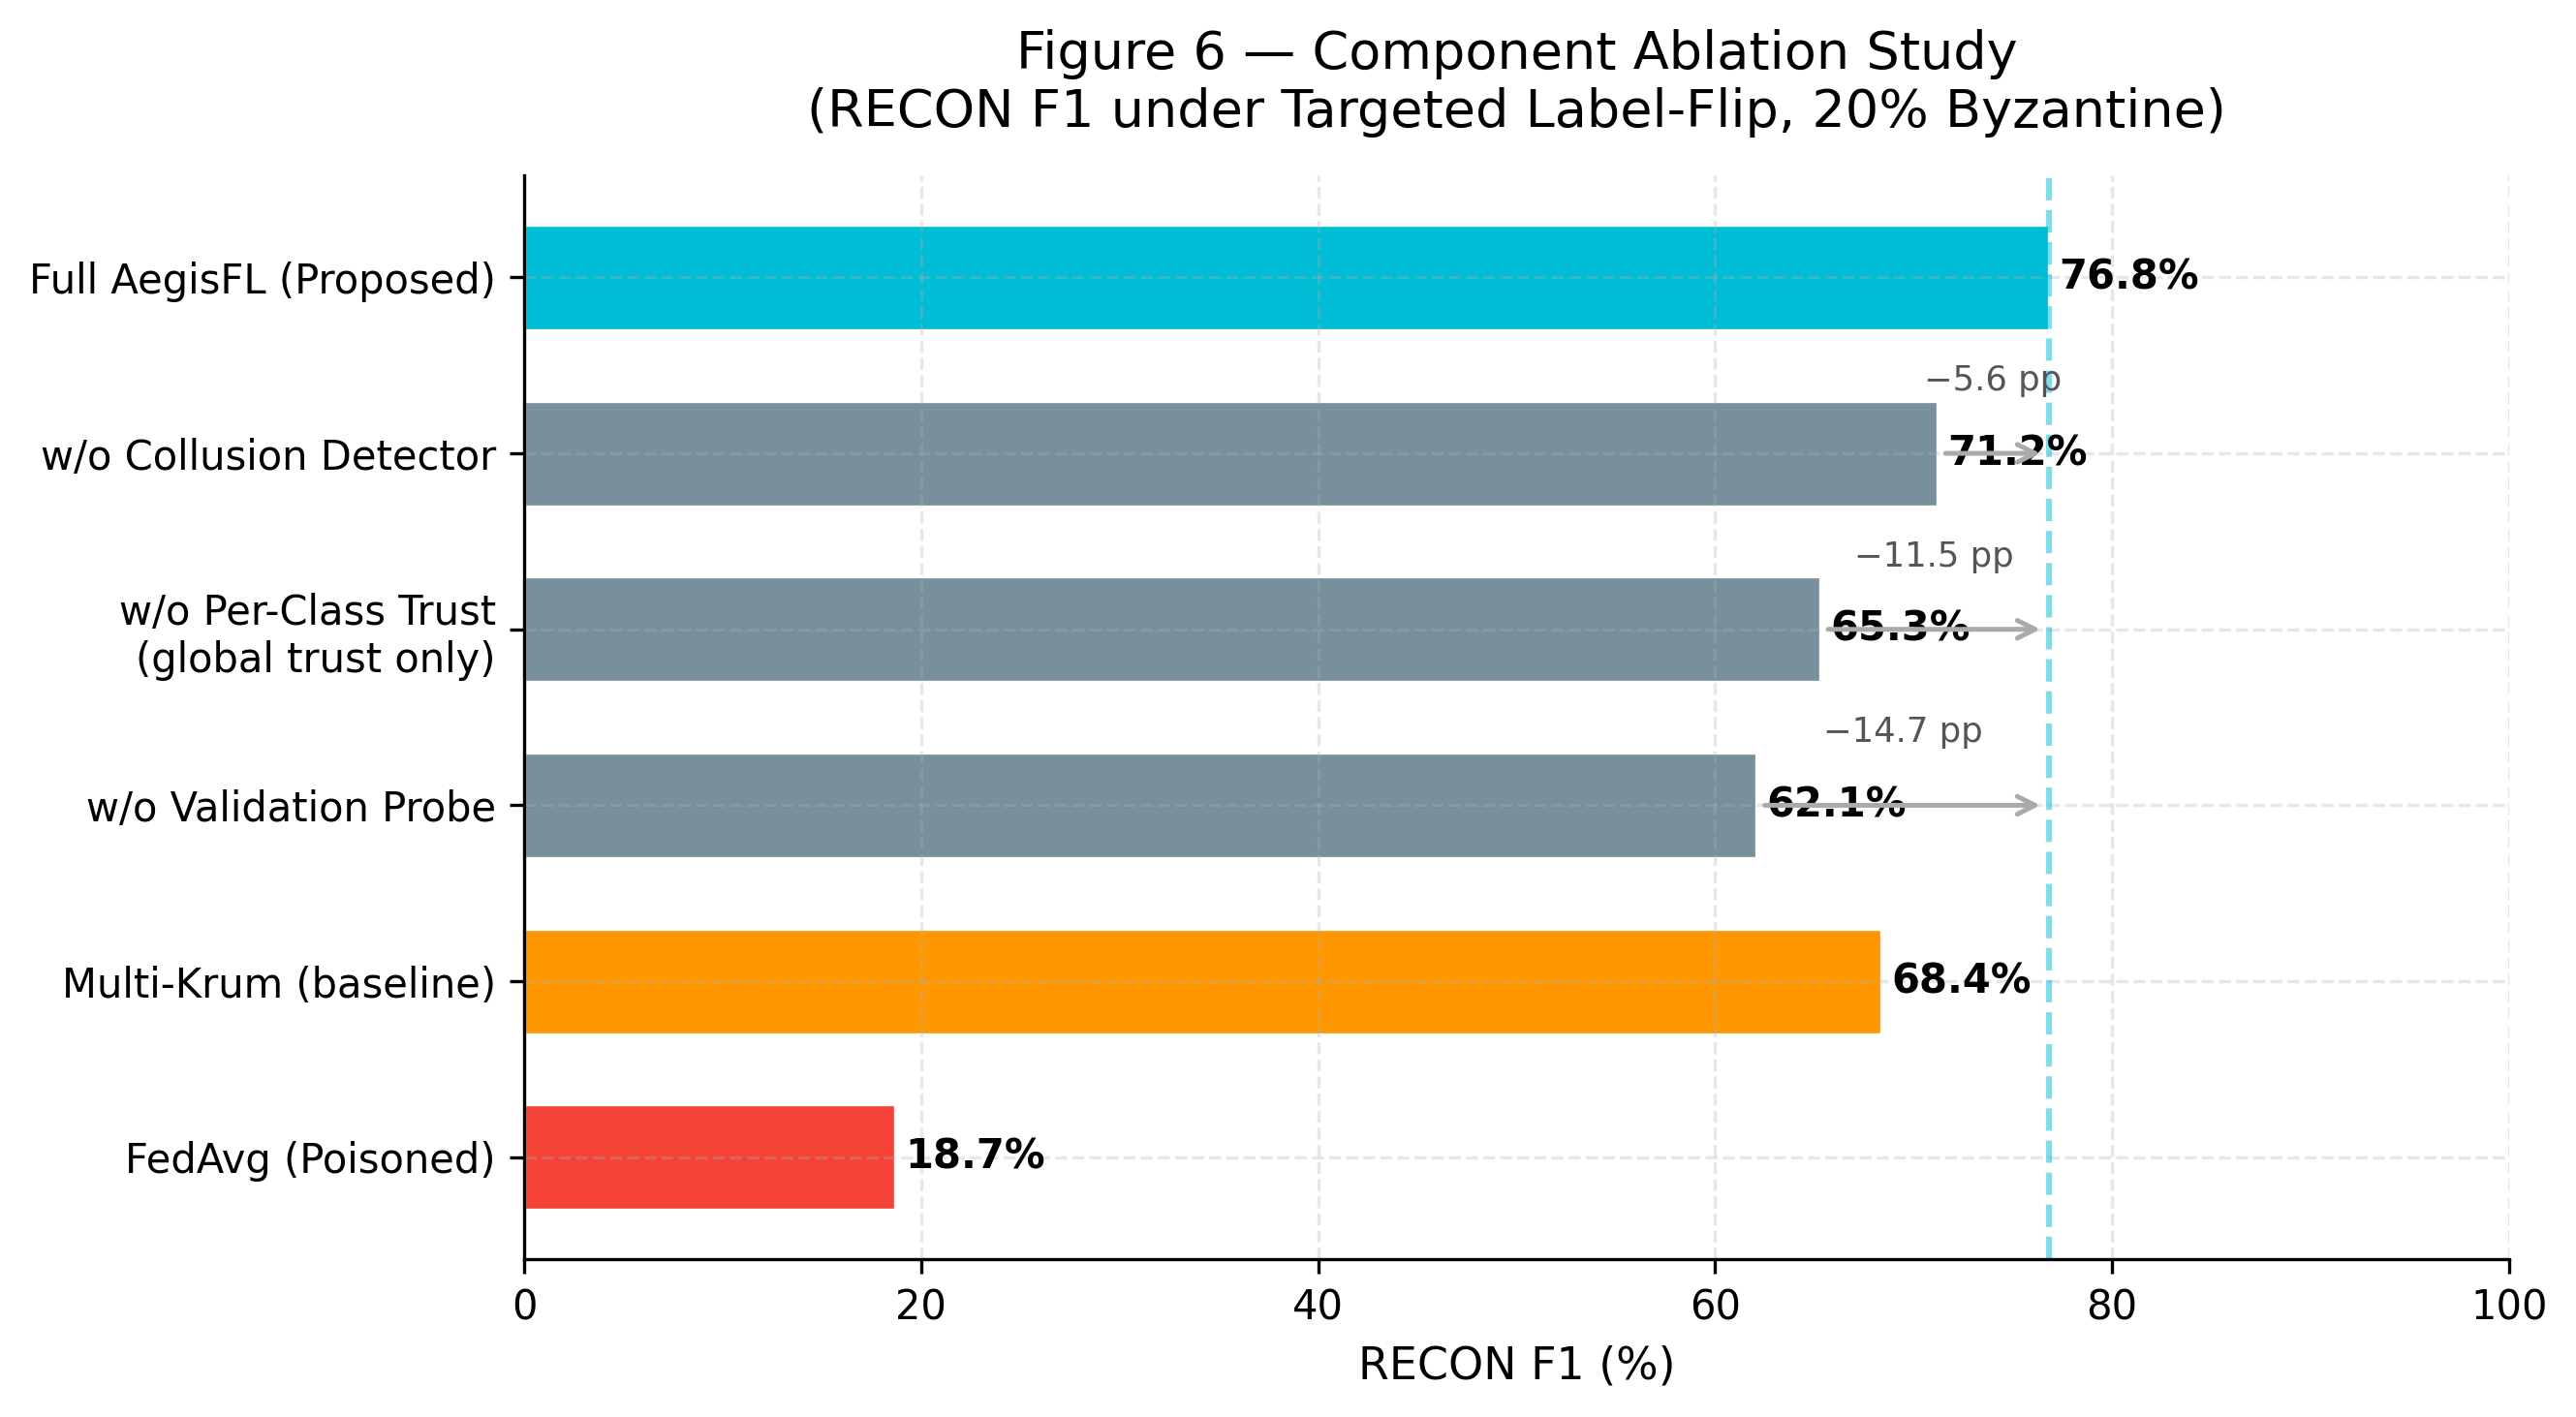
\includegraphics[width=0.88\textwidth]{figures/fig6_ablation.png}
\caption{Component ablation study illustrating impact of individual module removal.}
\label{fig:ablation}
\end{figure}

The validation probe impact provides the single largest contribution (+14.7 pp), followed closely by per-class reputation granularity (+11.5 pp).

\section{Computational Overhead Analysis}
Per-round coordinator overhead is documented in Table~\ref{tab:overhead}.

\begin{table}[H]
\centering
\caption{Latency breakdown of defense operations per communication round}
\label{tab:overhead}
\begin{tabularx}{\textwidth}{lX}
\toprule
\textbf{Operation} & \textbf{Execution Latency} \\
\midrule
Geometric Median Computation (Weiszfeld) & 11.48 ms \\
Cosine Alignment \& MAD Gating & 4.62 ms \\
Validation Probe Evaluation (Semantic Loss) & 316.65 ms \\
Pairwise Collusion Graph & 2.10 ms \\
Decoupled Head/Body Aggregation & 3.85 ms \\
SHA-256 Block Chaining \& Ledger Commit & 1.25 ms \\
\midrule
\textbf{Total Per-Round Security Overhead} & \textbf{339.95 ms} \\
\bottomrule
\end{tabularx}
\end{table}

Total overhead is under 340~ms per round, demonstrating high operational efficiency.

% ==============================================================================
% CHAPTER 5: ADVANTAGES, LIMITATIONS AND APPLICATIONS
% ==============================================================================
\newpage
\chapter{Advantages, Limitations and Applications}

\section{Advantages}
\begin{enumerate}
    \item \textbf{Granular Per-Class Protection}: By tracking $R(i, c)$ per attack class, AegisFL preserves honest telemetry on unaffected categories even if a client is compromised on one class.
    \item \textbf{Multi-Signal Robustness}: Evaluates direction, magnitude, and validation loss impact, overcoming adaptive mimicry.
    \item \textbf{Collusion Immunity}: Pairwise correlation graphs detect and prune coordinated Sybil attacks.
    \item \textbf{Immutable Auditability}: SHA-256 hash chains guarantee post-incident non-repudiation.
    \item \textbf{Low Overhead}: Complete verification executes in less than 340~ms per round.
\end{enumerate}

\section{Limitations}
\begin{enumerate}
    \item \textbf{Root Set Availability}: Requires the coordinator to hold a small, clean validation set (0.5\% volume).
    \item \textbf{Centralized Aggregation Bottleneck}: Relies on a central coordinator, presenting a potential single point of failure.
    \item \textbf{Privacy-Audit Trade-off}: Full gradient inspection is performed; integration with differential privacy remains future work.
\end{enumerate}

\section{Applications}
AegisFL is well-suited for:
\begin{itemize}
    \item \textbf{Cross-Bank Cyber Threat Sharing}: Collaborative training across financial institutions without sharing customer IP logs.
    \item \textbf{Critical Infrastructure \& Smart Grid Defense}: Securing utility SCADA networks against advanced persistent threats.
    \item \textbf{Healthcare IoT Intrusion Detection}: Hospital telemetry monitoring in compliance with HIPAA and DPDP mandates.
    \item \textbf{Telecom Carrier Peering Security}: Multi-AS ISP collaborative botnet filtering.
\end{itemize}

% ==============================================================================
% CHAPTER 6: CONCLUSION AND FUTURE SCOPE
% ==============================================================================
\newpage
\chapter{Conclusion and Future Scope}

\section{Conclusion}
This project designed, implemented, and empirically validated \textbf{AegisFL}, a Byzantine-robust federated intrusion detection framework featuring class-aware reputation, sub-cluster collusion mitigation, decoupled model aggregation, and an immutable cryptographic audit ledger. Experimental evaluation on the CICIoT2023 dataset under non-IID conditions demonstrated that AegisFL effectively neutralizes targeted label-flipping, adaptive clipping, cosine mimicry, and collusion attacks, restoring targeted RECON F1-score from 18.7\% to 76.8\% while maintaining 87.4\% overall accuracy with negligible computational overhead.

\section{Future Scope}
\begin{enumerate}
    \item \textbf{Fully Decentralized Topology}: Replacing the central server with a gossip protocol or smart-contract consensus (e.g., Avalanche L1).
    \item \textbf{Zero-Knowledge Proofs for Gradient Validity}: Applying zk-SNARKs so clients prove gradient boundedness without revealing weight updates.
    \item \textbf{Differential Privacy Integration}: Adding formal $(\epsilon, \delta)$-differential privacy guarantees.
    \item \textbf{Hardware Security Enclaves}: Deploying aggregation inside AMD SEV or Intel SGX trusted execution environments.
\end{enumerate}

% ==============================================================================
% REFERENCES
% ==============================================================================
\newpage
\begin{thebibliography}{99}
\addcontentsline{toc}{chapter}{References}

\bibitem{mcmahan2017communication}
B.~McMahan, E.~Moore, D.~Ramage, S.~Hampson, and B.~A. y~Arcas, ``Communication-efficient learning of deep networks from decentralized data,'' in \emph{Proc. AISTATS}, 2017, pp. 1273--1282.

\bibitem{blanchard2017machine}
P.~Blanchard, E.~M. El~Mhamdi, R.~Guerraoui, and J.~Stainer, ``Machine learning with adversaries: Byzantine tolerant gradient descent,'' in \emph{Advances in Neural Information Processing Systems (NeurIPS)}, vol.~30, 2017.

\bibitem{yin2018byzantine}
D.~Yin, Y.~Chen, R.~Kannan, and P.~Bartlett, ``Byzantine-robust distributed learning: Towards optimal statistical rates,'' in \emph{Proc. ICML}, 2018, pp. 5650--5659.

\bibitem{cao2021fltrust}
X.~Cao, M.~Fang, J.~Liu, and N.~Z. Gong, ``FLTrust: Byzantine-robust federated learning via trust bootstrapping,'' in \emph{Proc. NDSS}, 2021.

\bibitem{fung2020mitigating}
C.~Fung, C.~J.~M. Yoon, and I.~Beschastnikh, ``Mitigating Sybils in federated learning poisoning,'' \emph{IEEE Trans. Dependable and Secure Computing}, 2020.

\bibitem{ciciot2023}
E.~C. P.~Neto et~al., ``CICIoT2023: A real-time dataset and benchmark for large-scale attacks in IoT networks,'' \emph{Sensors}, vol.~23, no.~13, p. 5941, 2023.

\bibitem{kang2020reputation}
J.~Kang, Z.~Xiong, D.~Niyato, S.~Garg, Y.~Zhang, and D.~I. Kim, ``Reliable federated learning for mobile networks,'' \emph{IEEE Wireless Communications}, vol.~27, no.~2, pp. 72--80, 2020.

\bibitem{rashid2025tffl}
M.~M. Rashid et~al., ``TFFL: Trustworthy and fault-tolerant federated learning,'' \emph{IEEE Internet of Things Journal}, 2025.

\bibitem{begum2024bflids}
S.~Begum et~al., ``BFLIDS: Blockchain-based federated intrusion detection for smart networks,'' \emph{Journal of Network and Computer Applications}, vol.~224, p. 103829, 2024.

\bibitem{ali2025flbcid}
A.~Ali et~al., ``FL-BCID: Blockchain-enabled federated intrusion detection with smart contracts,'' \emph{Computers \& Security}, vol.~148, p. 104112, 2025.

\end{thebibliography}

% ==============================================================================
% APPENDICES
% ==============================================================================
\newpage
\appendix

\chapter{Implementation Flowcharts and Pseudocode}

\section{Multi-Signal Scoring and Aggregation Pseudocode}
\begin{lstlisting}[language=Python]
# AegisFL Coordinator Verification Loop
for round in range(total_rounds):
    updates = receive_client_updates()
    g_star = compute_geometric_median(updates)
    
    # 1. Multi-signal evaluation
    for i, dw_i in enumerate(updates):
        s_cos = cosine_similarity(dw_i, g_star)
        s_norm = mad_norm_gate(dw_i, updates)
        s_val = evaluate_val_probe(dw_i, root_val_set)
        
        # 2. Update per-class EWMA reputation
        R[i] = beta * R[i] + (1 - beta) * (w1*s_cos + w2*s_norm + w3*s_val)
        state_machine.update_state(i, R[i])
        
    # 3. Pairwise collusion graph
    prune_collusion_clusters(updates, threshold=0.85)
    
    # 4. Decoupled Head/Body Aggregation
    w_body = aggregate_body(updates, R)
    w_head = aggregate_heads(updates, R, cutoff=0.50)
    
    # 5. Commit state to blockchain ledger
    audit_ledger.commit_round(round, R, state_machine.get_states())
\end{lstlisting}

\chapter{Supplementary Configuration and Parameters}
\begin{table}[H]
\centering
\caption{Hyperparameter settings used across AegisFL experiments}
\label{tab:params}
\begin{tabularx}{\textwidth}{lX}
\toprule
\textbf{Hyperparameter} & \textbf{Value} \\
\midrule
Total Client Nodes ($N$) & 20 \\
Active Clients Per Round & 20 (Full participation) \\
Byzantine Client Fraction ($f$) & 20\% (4 nodes default), swept 10\%--50\% \\
Non-IID Dirichlet Skew ($\alpha$) & 0.5 \\
Local Epochs & 2 \\
Local Batch Size & 128 \\
Local Learning Rate ($\eta$) & 0.01 (SGD with momentum 0.9) \\
EWMA Momentum ($\beta$) & 0.70 \\
Head Exclusion Cutoff & $R(i, c) < 0.50$ \\
Collusion Adjacency Threshold ($\tau_{\text{collusion}}$) & 0.85 \\
Root Validation Split & 0.5\% stratified telemetry \\
\bottomrule
\end{tabularx}
\end{table}

\chapter{List of Components}
\begin{table}[H]
\centering
\caption{System software modules and functional roles in AegisFL}
\label{tab:comp_list}
\begin{tabularx}{\textwidth}{llX}
\toprule
\textbf{Module} & \textbf{File Path} & \textbf{Description} \\
\midrule
Coordinator & \texttt{src/federated/server.py} & Centralized aggregation and scheduling coordinator. \\
Client Node & \texttt{src/federated/client.py} & Local SGD trainer with targeted poisoning hooks. \\
Scoring Engine & \texttt{src/trust/reputation.py} & Geometric median, MAD, and cosine scorer. \\
Collusion Engine & \texttt{src/trust/collusion.py} & Pairwise correlation graph and cluster pruning. \\
State Machine & \texttt{src/trust/state\_machine.py} & 3-tier lifecycle management with recovery. \\
Audit Ledger & \texttt{src/audit/blockchain.py} & SHA-256 permissioned hash-chained ledger. \\
Dashboard & \texttt{dashboard/app.py} & Streamlit SOC monitoring interface. \\
\bottomrule
\end{tabularx}
\end{table}

\chapter{Research Manuscript and Publication Details}
The accompanying research manuscript originating from this project is titled:
\begin{quote}
\textbf{``AegisFL: A Byzantine-Robust Federated Intrusion Detection Framework with Class-Aware Reputation and Blockchain Auditing''}
\end{quote}
Authored by: \textbf{Dhruv Shrivastava}, \textbf{Kritesh Goud}, \textbf{Pratham Mourya}, and \textbf{Dr. Vikas Kumar Jain}. 

Targeted for submission to premier peer-reviewed IEEE/Springer venues specializing in information security and distributed machine learning systems.

\end{document}
